% Slide1: Introduction -----------------------------------------------------------

% FIXME R vs A -  I guess change to A (A is used for implicit
% assumption slides.. so fix this!)




\begin{frame}
  \centerline{
\includegraphics[height=0.7\textheight]{images/cail.png}}
  \centerline{http://cail.criteo.com}
\end{frame}



\begin{frame}[fragile]
  \frametitle{Notation}

\begin{table}
  \begin{tabular}{c l r}
    \toprule
    \textbf{Symbol} & \textbf{Dimension} & \textbf{Description} \\ 
    \midrule
    \midrule
    $u$ & Scalar & A given users id.  \\
    $t$ & Scalar & sequential time. \\%, an integer indicating item occurrence.\\
    $P$ & Scalar & Total number of products. \\
    $v_{t}$ & Scalar & Product id viewed by user at time $t$.\\
    $r_{t}$ & Scalar & Product id recommended at time $t$.\\
    $c_{t}$ & Scalar & Product id recommended at time $t$.  \\  
    \bottomrule    
    \end{tabular}
    \caption{Notations and Definitions} 
    \vskip -15pt
    \label{tab:notation}
  \end{table}
\end{frame}



\begin{frame}
  \frametitle{Classic Reco}
 
 
   \begin{figure}[h!]
     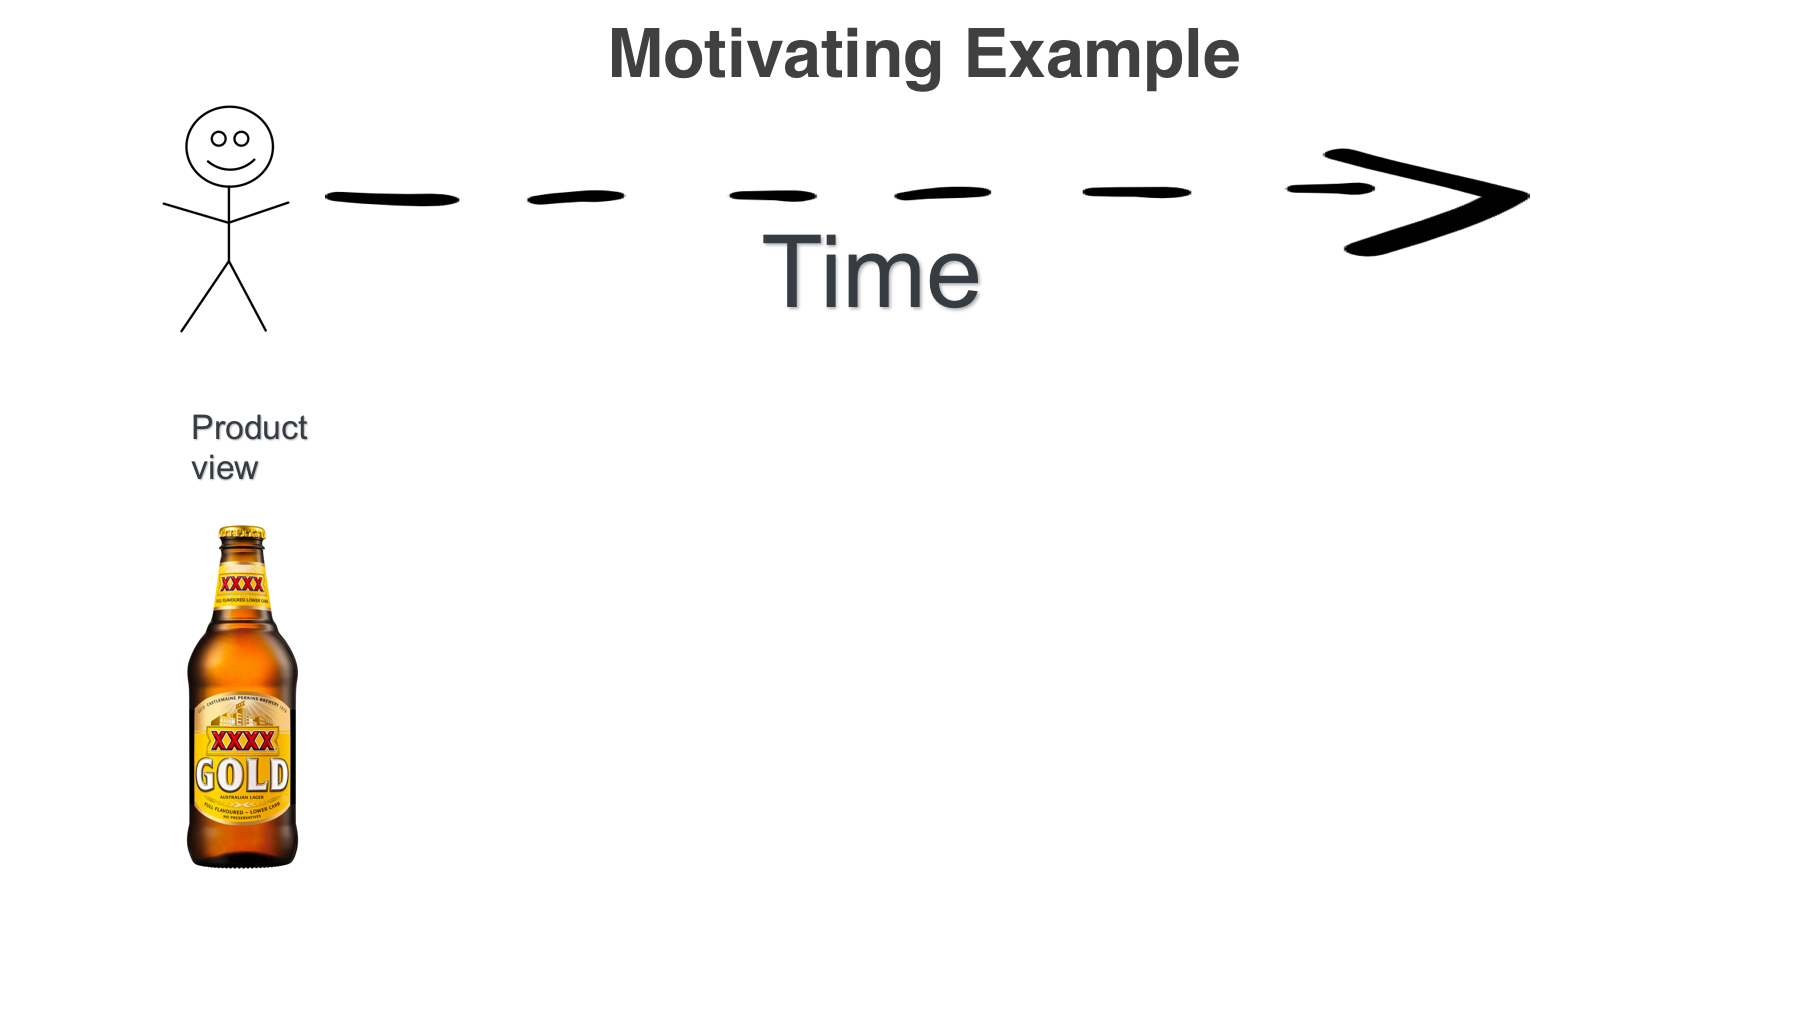
\includegraphics[scale=0.25]{images/mot_ex1a.png}
       \centering
       \label{motex1}
   \end{figure}
     
 \end{frame}


\begin{frame}
  \frametitle{Classic Reco}
 
 
   \begin{figure}[h!]
     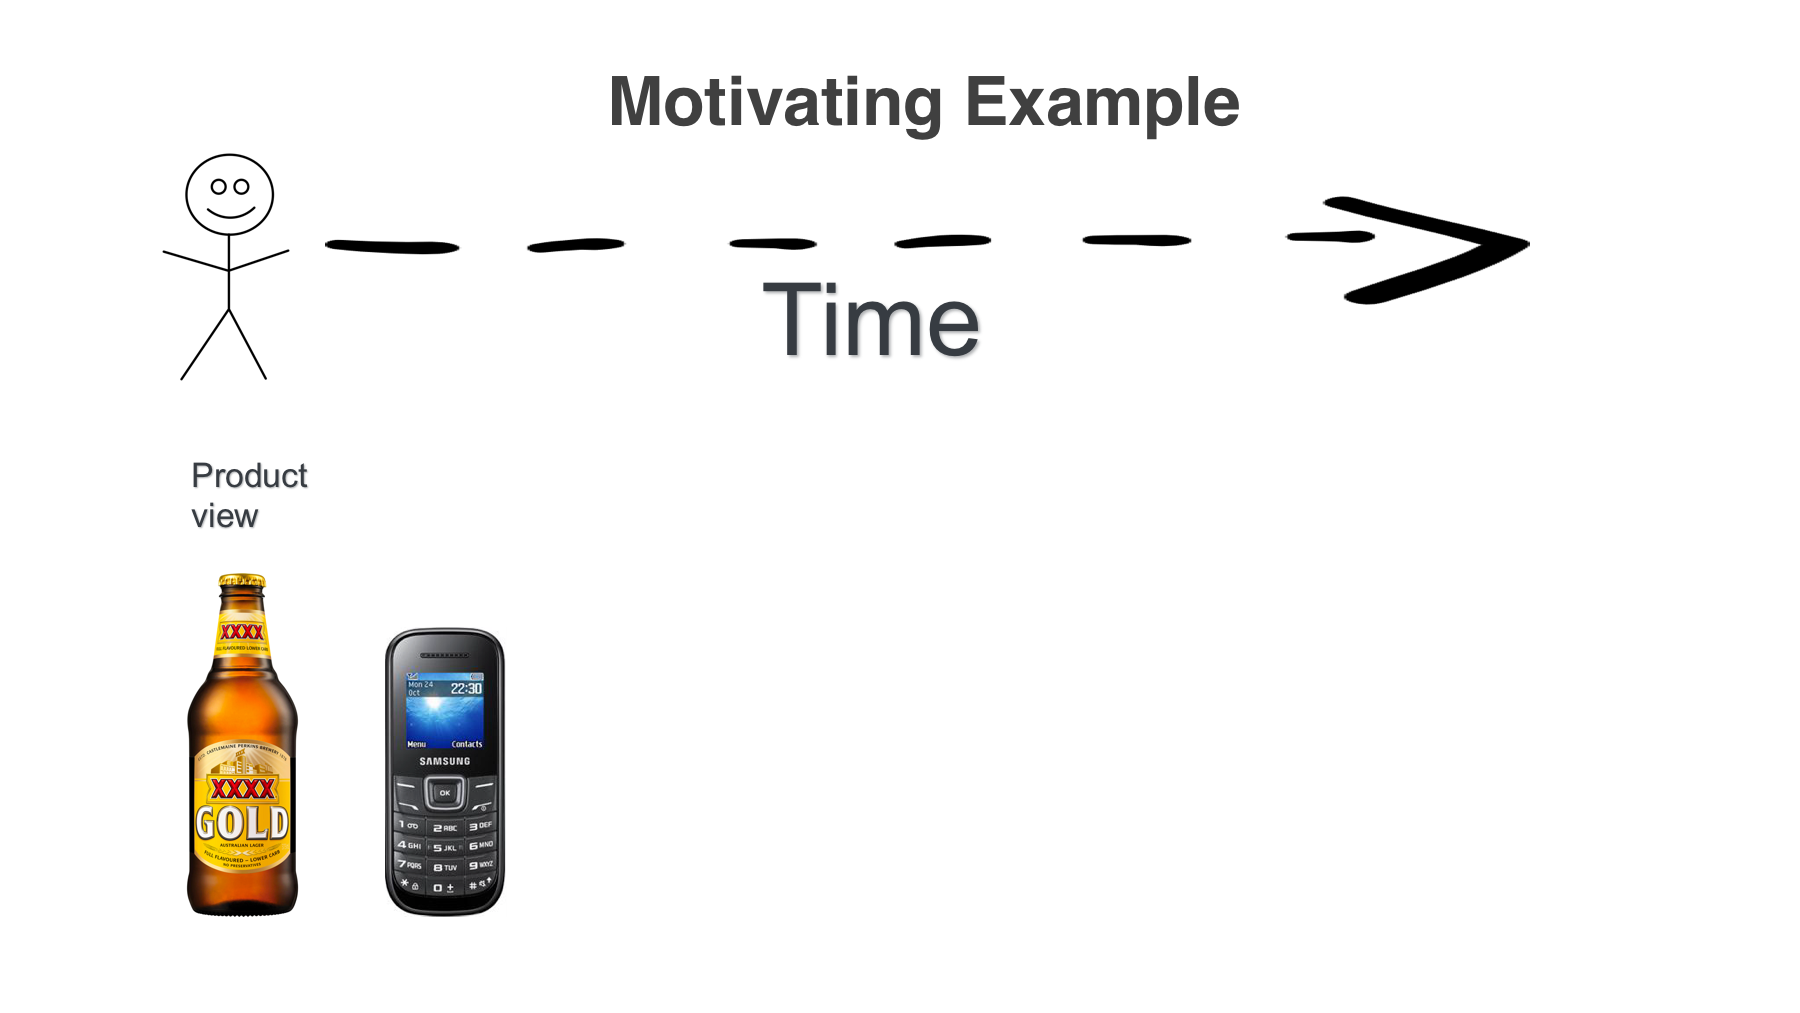
\includegraphics[scale=0.25]{images/mot_ex1b.png}
       \centering
       \label{motex1}
   \end{figure}
     
 \end{frame}


\begin{frame}
  \frametitle{Classic Reco}
 
 
   \begin{figure}[h!]
     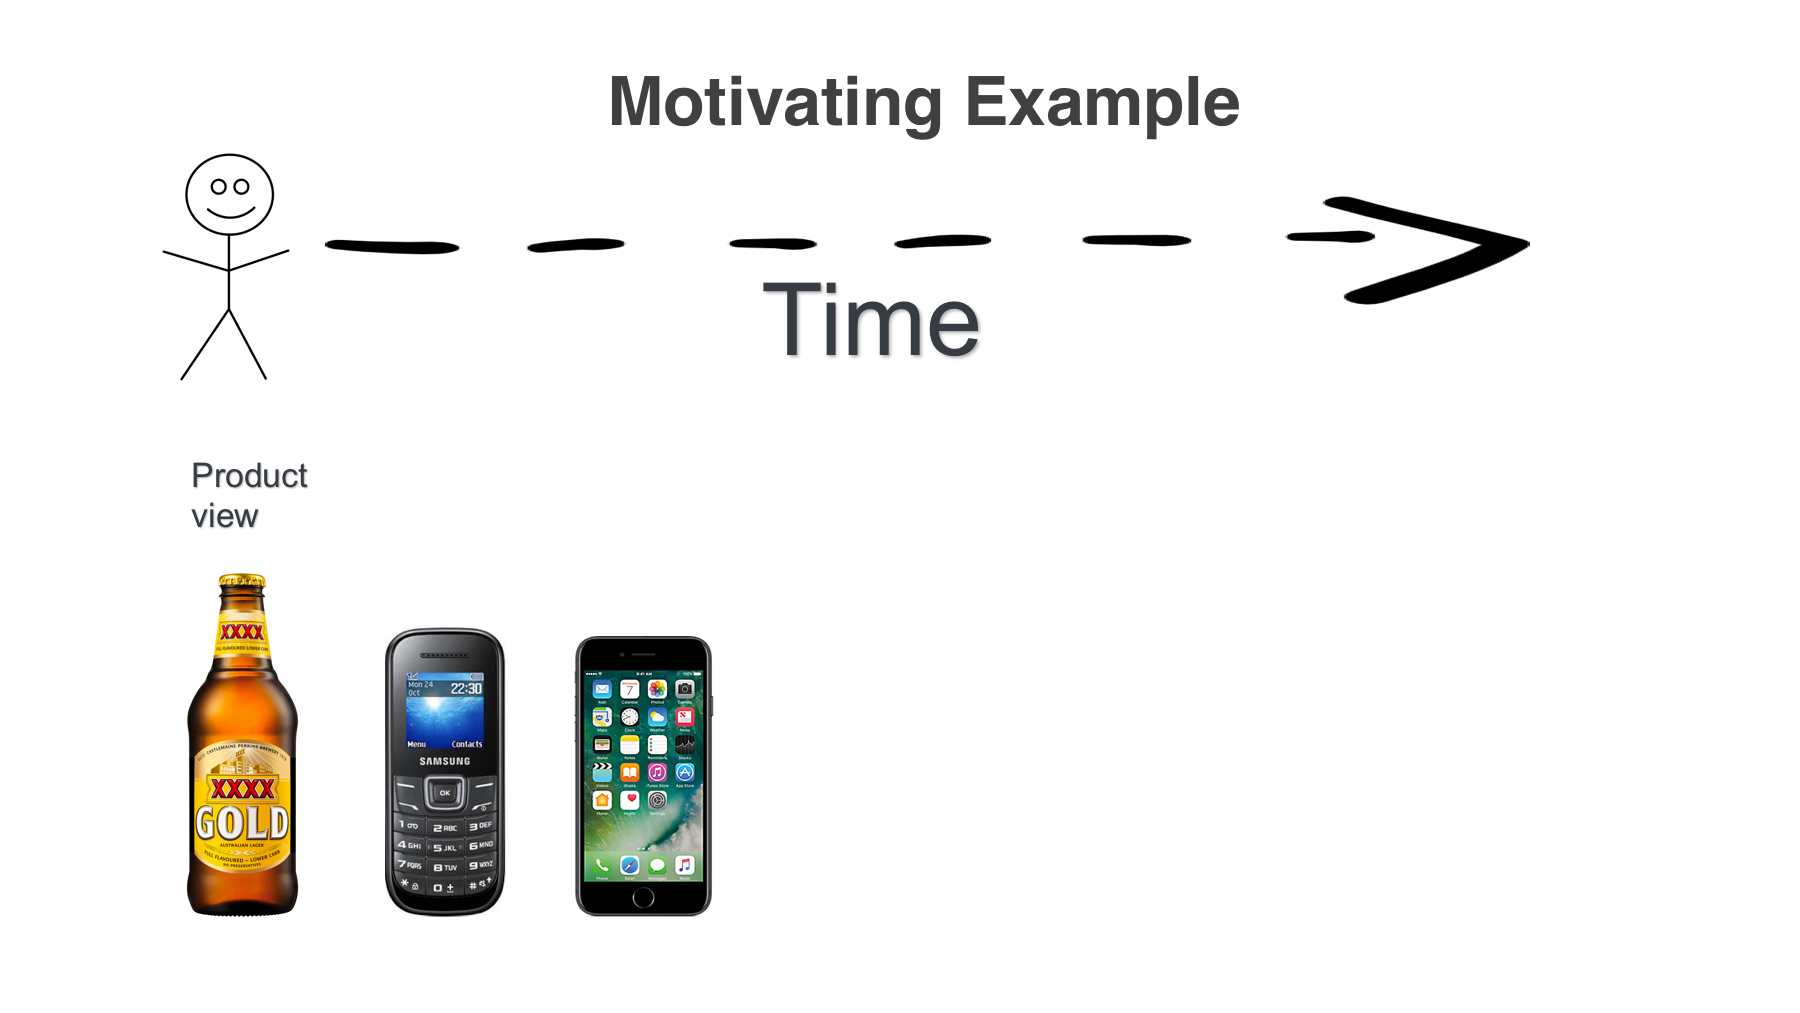
\includegraphics[scale=0.25]{images/mot_ex1cc.png}
       \centering
       \label{motex1}
   \end{figure}
     
 \end{frame}




 \begin{frame}
  \frametitle{Classic Reco}
 
 
   \begin{figure}[h!]
     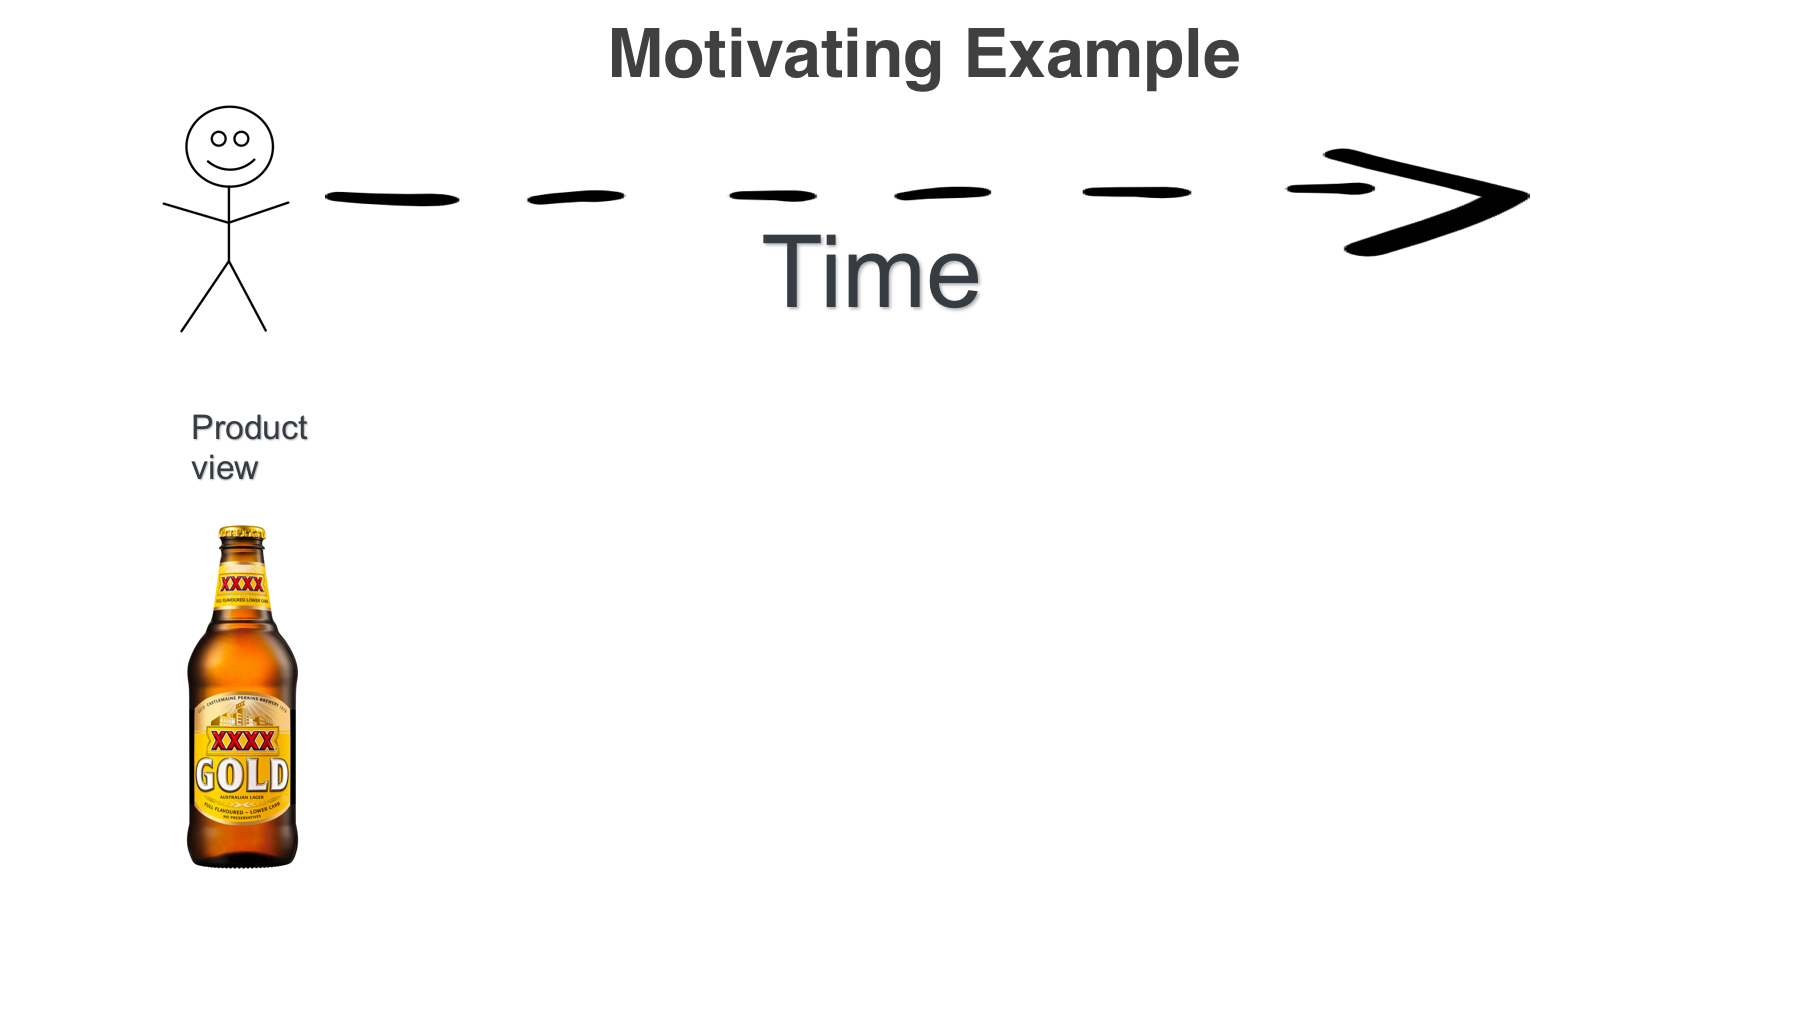
\includegraphics[scale=0.25]{images/mot_ex1a.png}
       \centering
       \label{motex1}
   \end{figure}

   \[
   P(V_1 = {\rm beer})  
   \]
 \end{frame}


\begin{frame}
  \frametitle{Classic Reco}
 
 
   \begin{figure}[h!]
     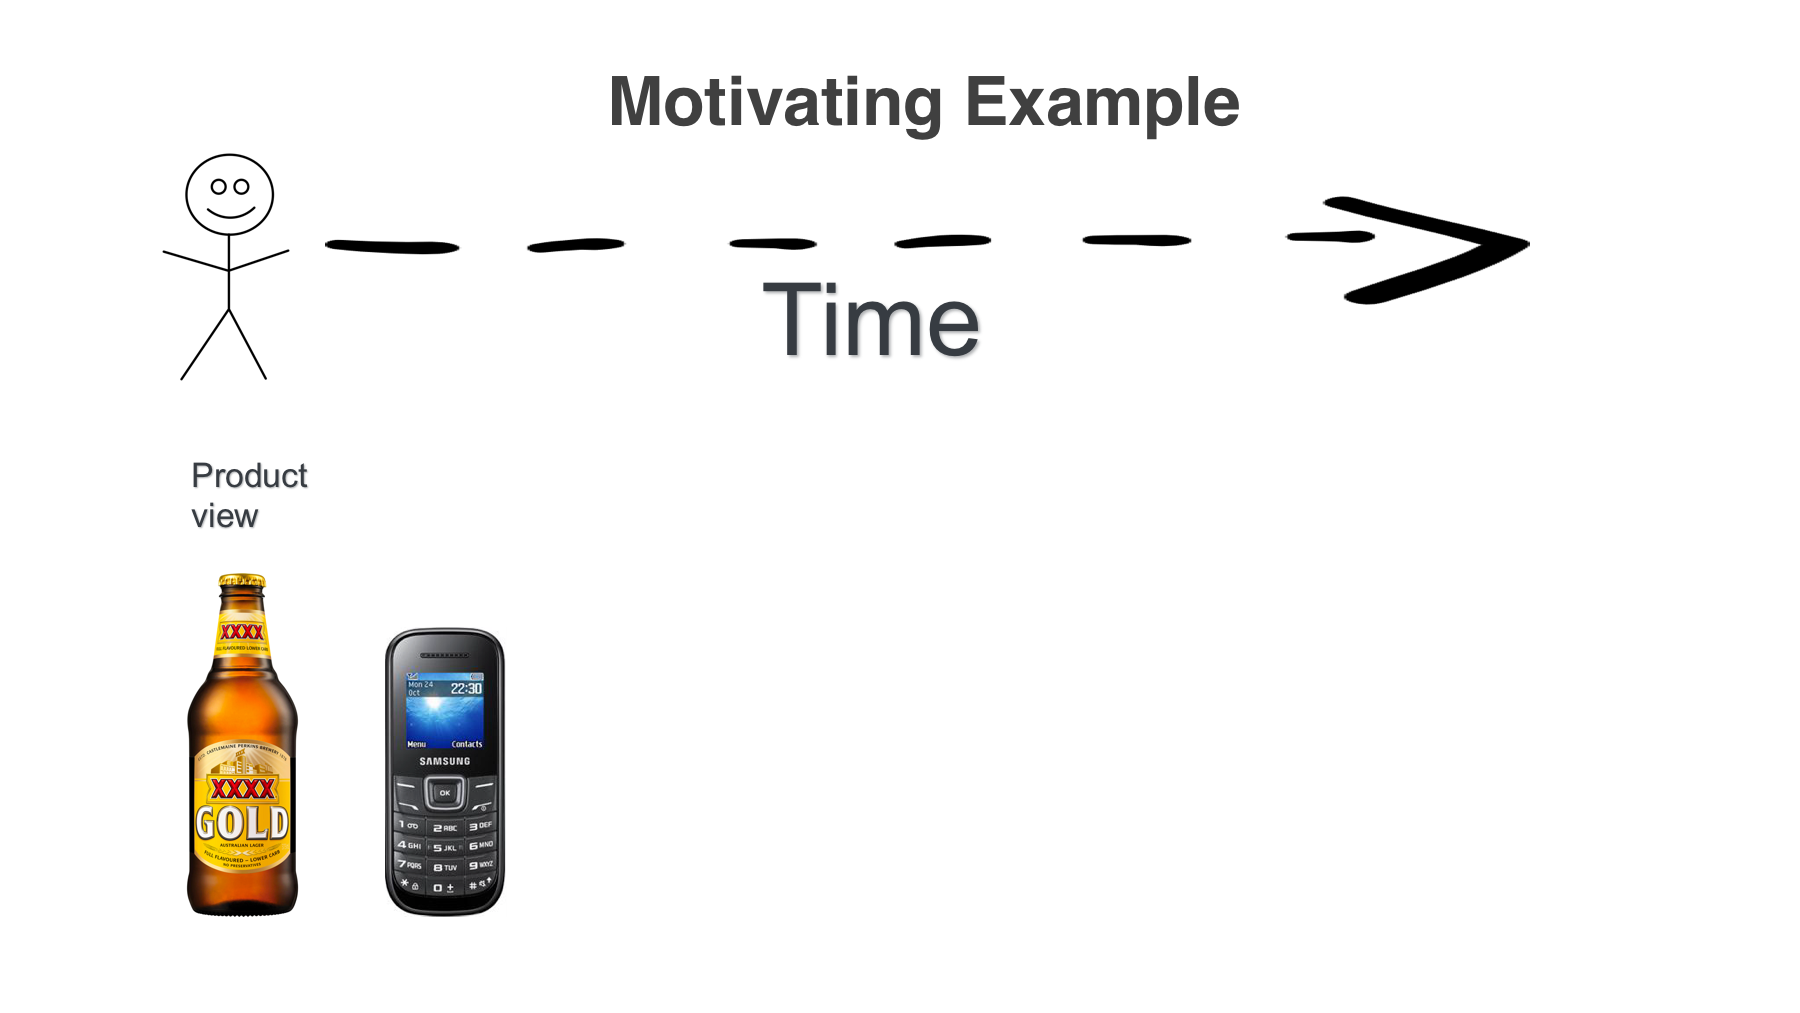
\includegraphics[scale=0.25]{images/mot_ex1b.png}
       \centering
       \label{motex1}
   \end{figure}
   \[
   P(V_2 = {\rm phone ~ A} | V_1 = {\rm beer})  
   \]
     
 \end{frame}


\begin{frame}
  \frametitle{Classic Reco}
 
 
   \begin{figure}[h!]
     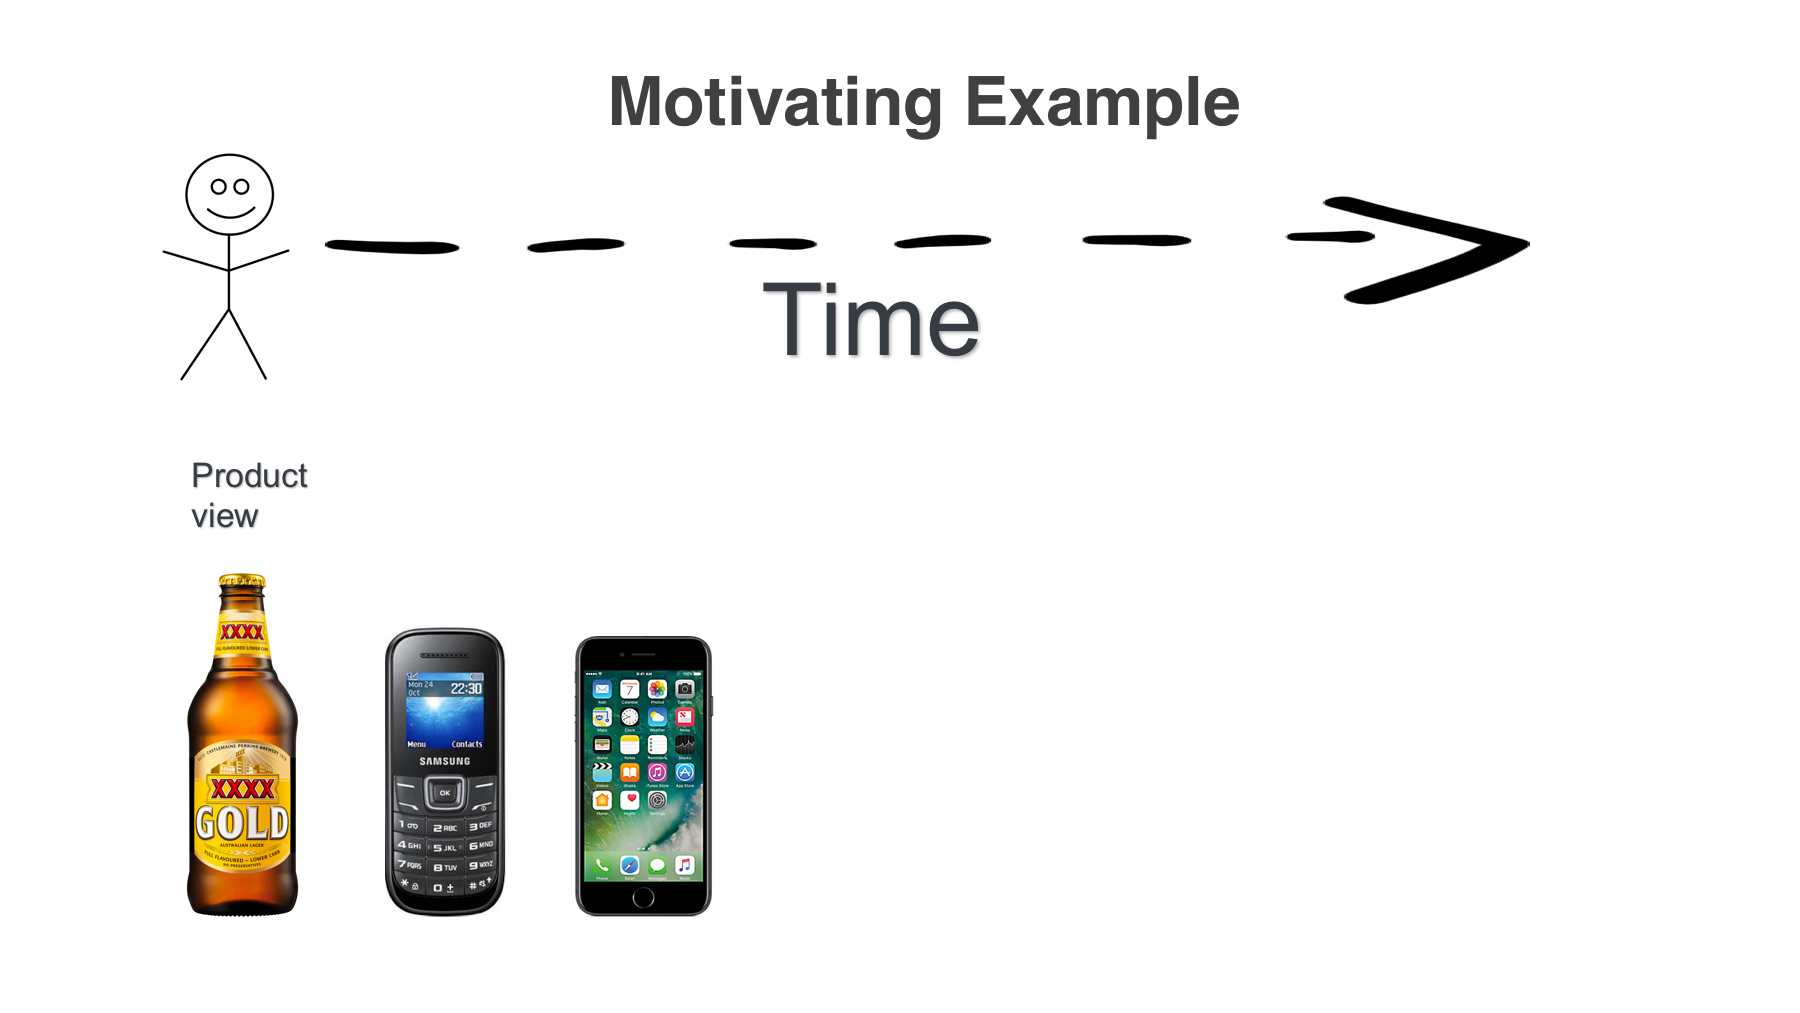
\includegraphics[scale=0.25]{images/mot_ex1cc.png}
       \centering
       \label{motex1}
   \end{figure}

   \[
   P(V_3 = {\rm phone ~ B} | V_1 = {\rm beer}, V_2 = {\rm phone ~ A} )  
   \]

   
 \end{frame}



 \begin{frame}
  \frametitle{Next Item Prediction, hold out $V_3$}

  \begin{tabular}{r r}
    $P(V_3 = {\rm phone ~ A} | V_1 = {\rm beer}, V_2 = {\rm phone ~ A} )$ &= $0.27$ \\
    $P(V_3 = {\rm phone ~ B} | V_1 = {\rm beer}, V_2 = {\rm phone ~ A} )$ &= $0.24$ \\
    $P(V_3 = {\rm rice} | V_1 = {\rm beer}, V_2 = {\rm phone ~ A} )$ &= $0.10$ \\
    $P(V_3 = {\rm couscous} | V_1 = {\rm beer}, V_2 = {\rm phone ~ A} )$ &= $0.09$ \\
    $P(V_3 = {\rm beer} | V_1 = {\rm beer}, V_2 = {\rm phone ~ A} )$ &= $0.30$ \\
  \end{tabular}


\vspace{4mm}  
  \pause
What actually happened? \pause $V_3 = {\rm phone ~ B} $

\vspace{4mm}  
  \pause
Our model assigned: $P(V_3 = {\rm phone ~ B} | V_1 = {\rm beer}, V_2 = {\rm phone ~ A}) = 0.24$ 

\pause
Of course better would be higher, but how good is this?

 \end{frame}



 \begin{frame}
  \frametitle{Next Item Prediction, hold out $V_3$: Log likelihood}

What actually happened? \pause $V_3 = {\rm phone ~ B} $

\vspace{4mm}  
  \pause
Our model assigned: $P(V_3 = {\rm phone ~ B} | V_1 = {\rm beer}, V_2 = {\rm phone ~ A}) = 0.24$ 

\vspace{4mm}  

\pause
Log Likelihood:
$\log P(V_3 = {\rm phone ~ B} | V_1 = {\rm beer}, V_2 = {\rm phone ~ A}) = -1.427116$ 

\vspace{4mm}  

\pause
Rationale:  you want to assign high values to things that happend.

 \end{frame}




 \begin{frame}
  \frametitle{Next Item Prediction, hold out $V_3$: HR@K Recall@K
    Precision@K - K=2}

  \begin{tabular}{r r}
    $P(V_3 = {\rm phone ~ A} | V_1 = {\rm beer}, V_2 = {\rm phone ~ A} )$ &= $0.27$ \\
    $P(V_3 = {\rm phone ~ B} | V_1 = {\rm beer}, V_2 = {\rm phone ~ A} )$ &= $0.24$ \\
    $P(V_3 = {\rm rice} | V_1 = {\rm beer}, V_2 = {\rm phone ~ A} )$ &= $0.10$ \\
    $P(V_3 = {\rm couscous} | V_1 = {\rm beer}, V_2 = {\rm phone ~ A} )$ &= $0.09$ \\
    $P(V_3 = {\rm beer} | V_1 = {\rm beer}, V_2 = {\rm phone ~ A} )$ &= $0.30$ \\
  \end{tabular}

  What actually happened? \pause $V_3 = {\rm phone ~ B} $


  \vspace{4mm}  
  \pause
Our model assigned: $P(V_3 = {\rm phone ~ B} | V_1 = {\rm beer}, V_2 = {\rm phone ~ A}) = 0.24$, which is 3rd place

How good is 3rd place?
\pause
HR@K if K=2, our model assigned phone B the third highest spot so it just misses out.

\vspace{4mm}  


 \end{frame}


 \begin{frame}
  \frametitle{Next Item Prediction, hold out $V_3$: HR@K Recall@K
    Precision@K - K=3}

  \begin{tabular}{r r}
    $P(V_3 = {\rm phone ~ A} | V_1 = {\rm beer}, V_2 = {\rm phone ~ A} )$ &= $0.27$ \\
    $P(V_3 = {\rm phone ~ B} | V_1 = {\rm beer}, V_2 = {\rm phone ~ A} )$ &= $0.24$ \\
    $P(V_3 = {\rm rice} | V_1 = {\rm beer}, V_2 = {\rm phone ~ A} )$ &= $0.10$ \\
    $P(V_3 = {\rm couscous} | V_1 = {\rm beer}, V_2 = {\rm phone ~ A} )$ &= $0.09$ \\
    $P(V_3 = {\rm beer} | V_1 = {\rm beer}, V_2 = {\rm phone ~ A} )$ &= $0.30$ \\
  \end{tabular}

  What actually happened? \pause $V_3 = {\rm phone ~ B} $


  \vspace{4mm}  
  \pause
Our model assigned: $P(V_3 = {\rm phone ~ B} | V_1 = {\rm beer}, V_2 = {\rm phone ~ A}) = 0.24$, which is 3rd place

How good is 3rd place?
\pause
HR@K if K=3, our model assigned phone B the third highest spot so it
is in.

\vspace{4mm}  

\pause
Rationale:  you want a ranking that assigns high positions to events that occur.  The position matters more than the probability.

 \end{frame}







 \begin{frame}
  \frametitle{Real Reco}
 
 
   \begin{figure}[h!]
     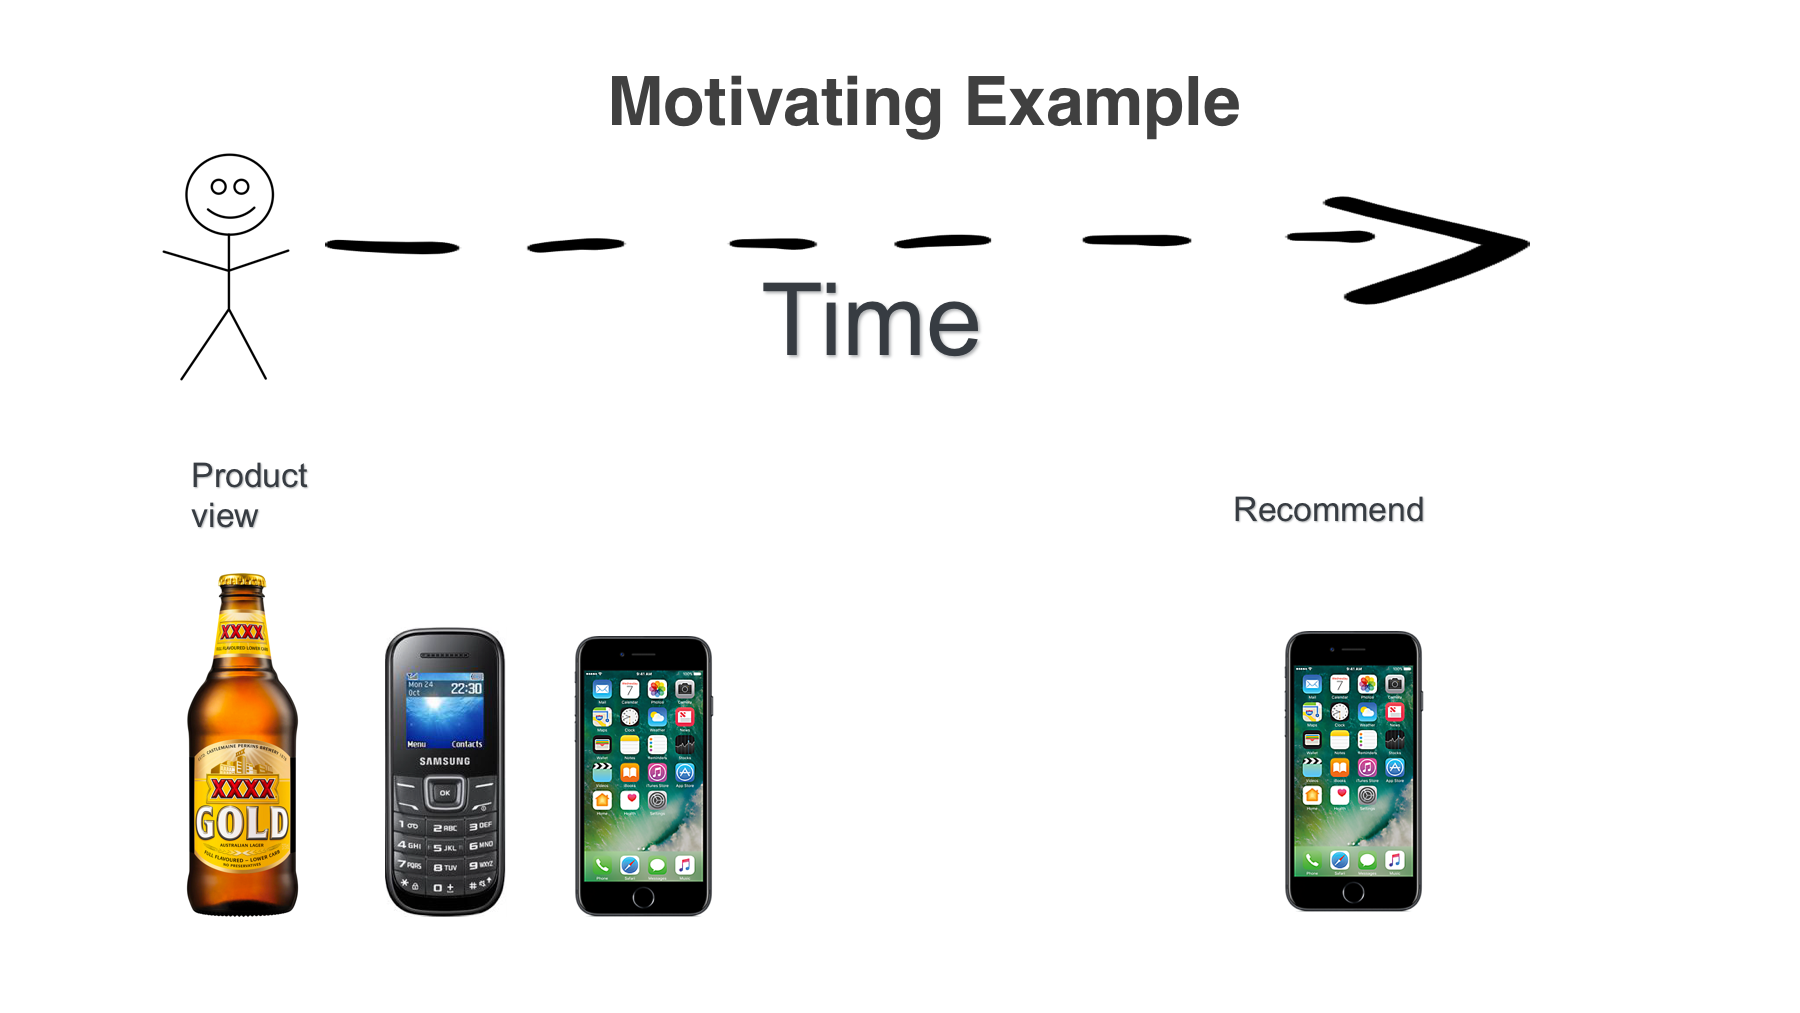
\includegraphics[scale=0.25]{images/mot_ex2.png}
       \centering
       \label{motex1}
   \end{figure}
     
 \end{frame}

 \begin{frame}
  \frametitle{Real Reco}
 
 
   \begin{figure}[h!]
     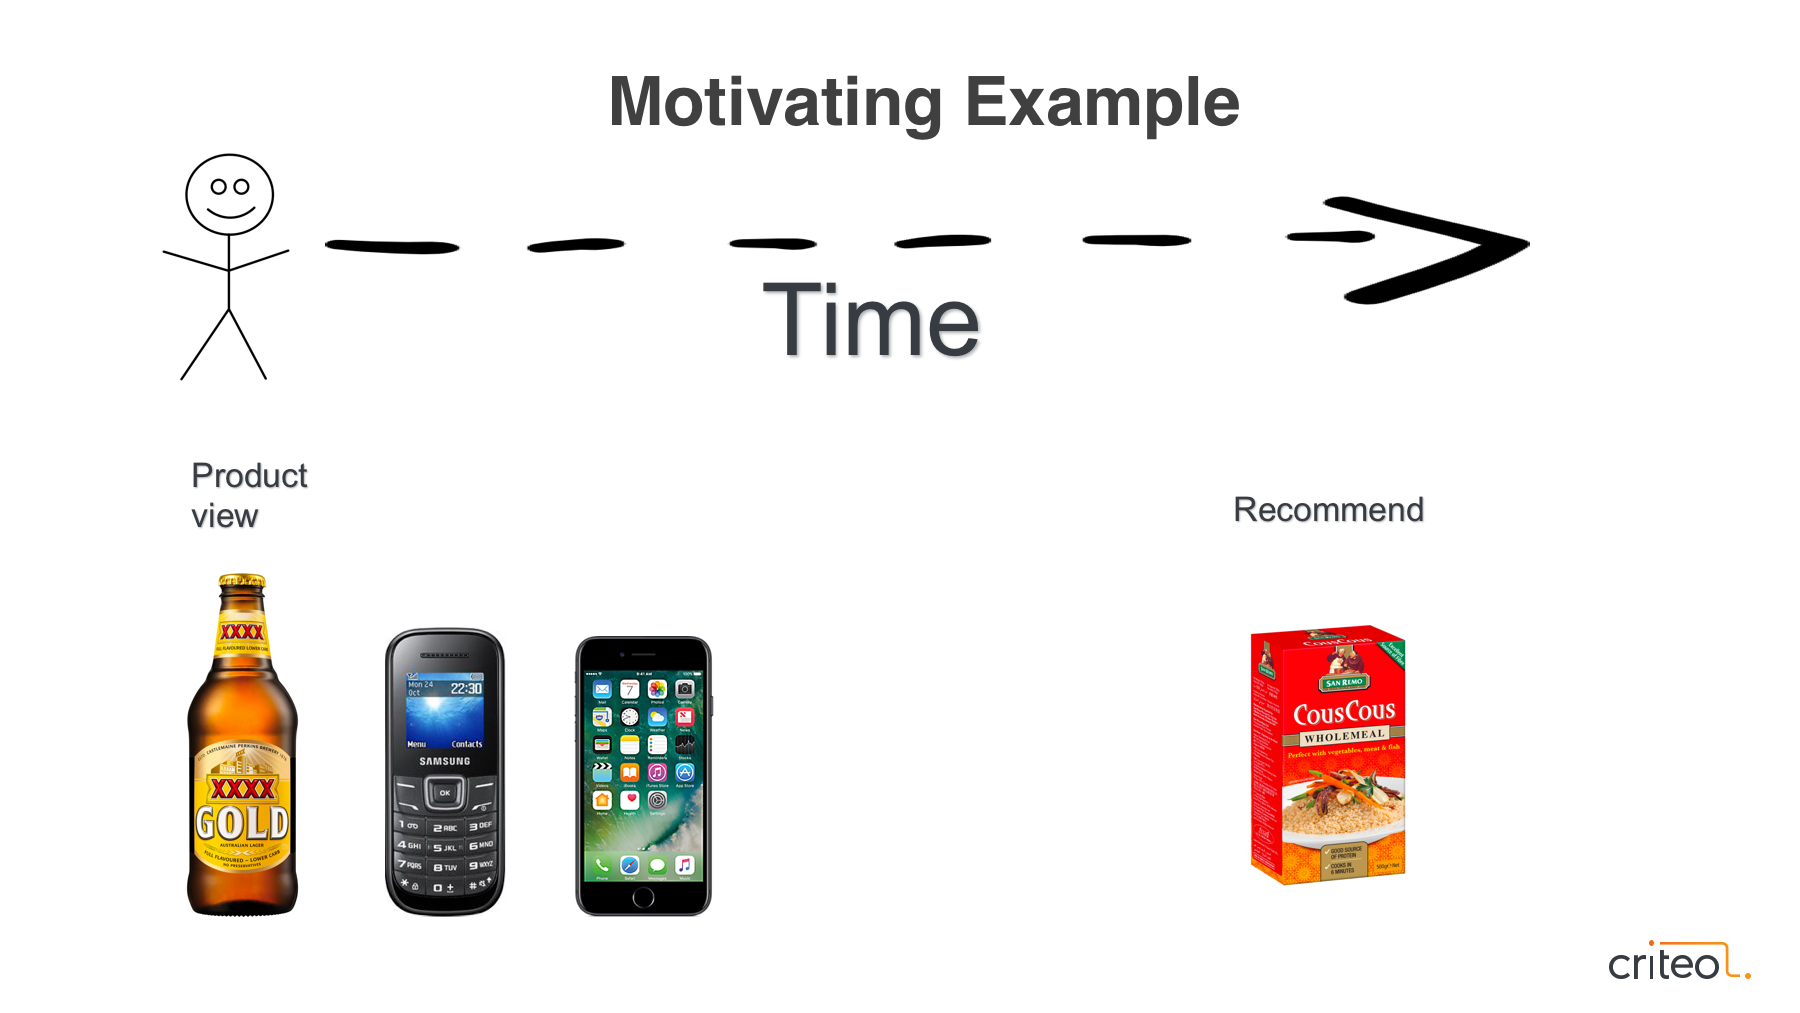
\includegraphics[scale=0.25]{images/mot_ex3.png}
       \centering
       \label{motex1}
   \end{figure}
     
 \end{frame}

 \begin{frame}
  \frametitle{Real Reco}
 
 
   \begin{figure}[h!]
     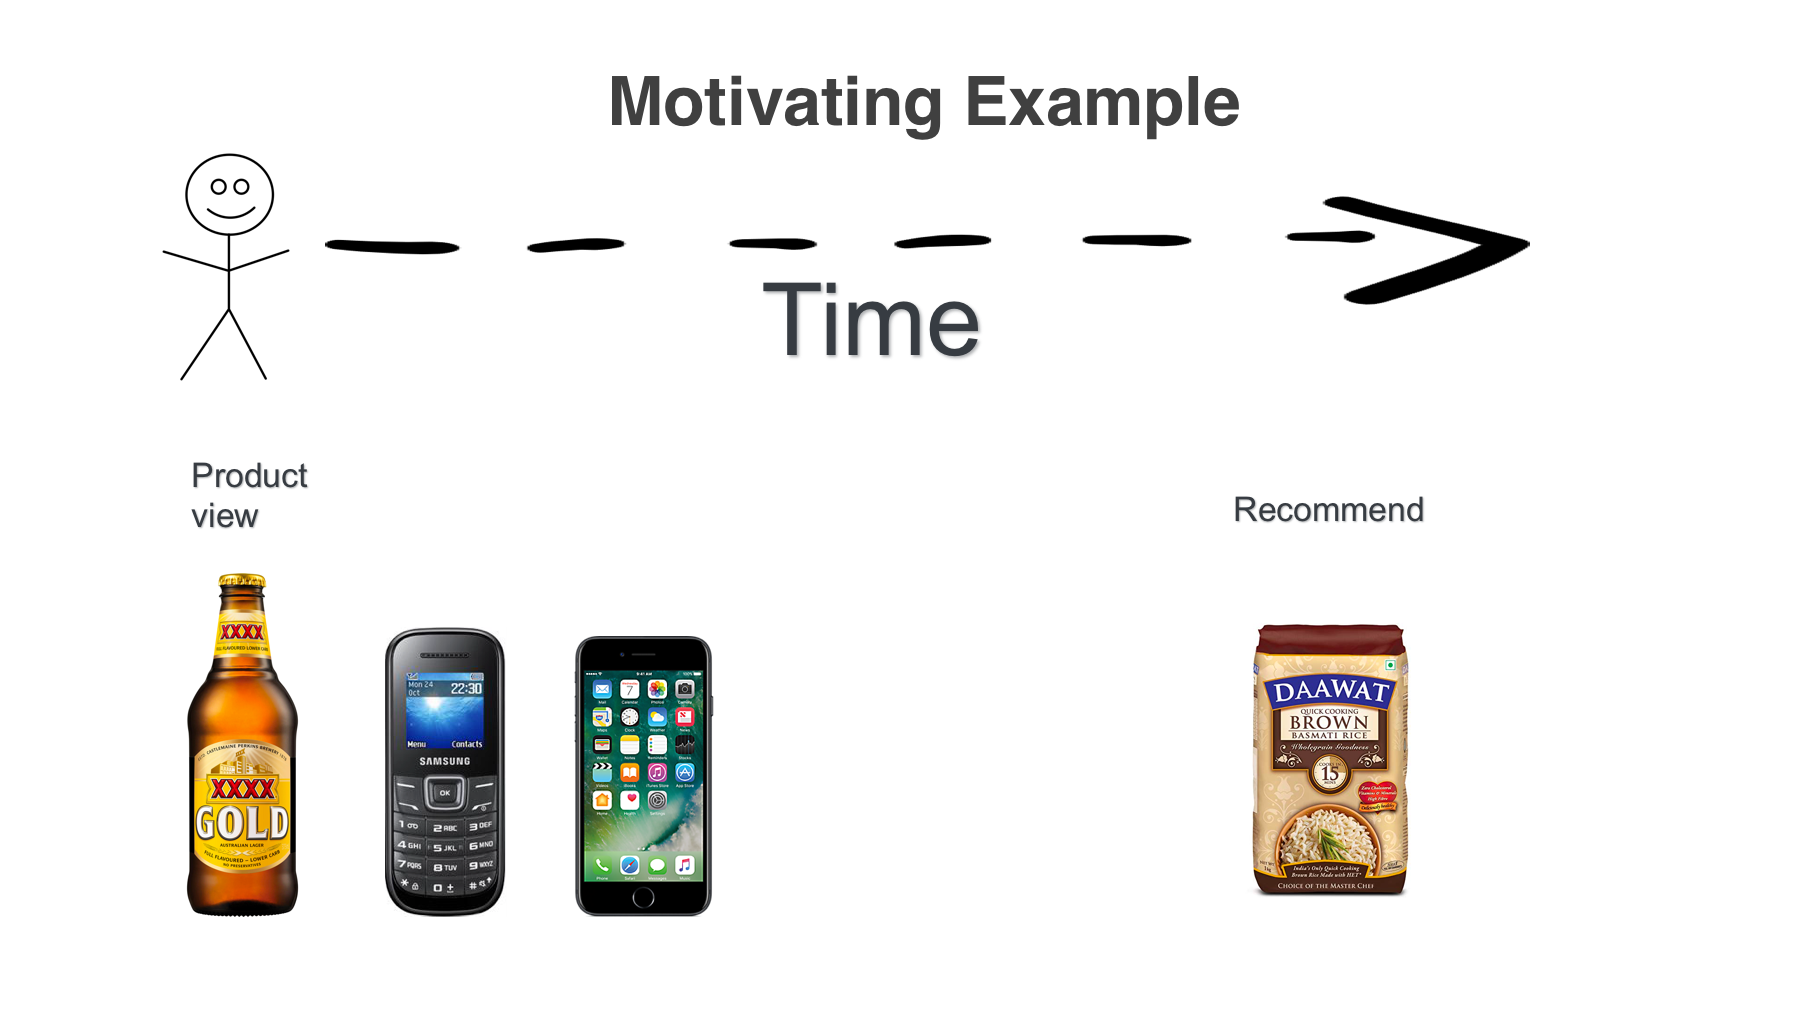
\includegraphics[scale=0.25]{images/mot_ex4.png}
       \centering
       \label{motex1}
   \end{figure}
     
 \end{frame}



 %%



 \begin{frame}
  \frametitle{The Real Reco Problem}
 
 
   \begin{figure}[h!]
     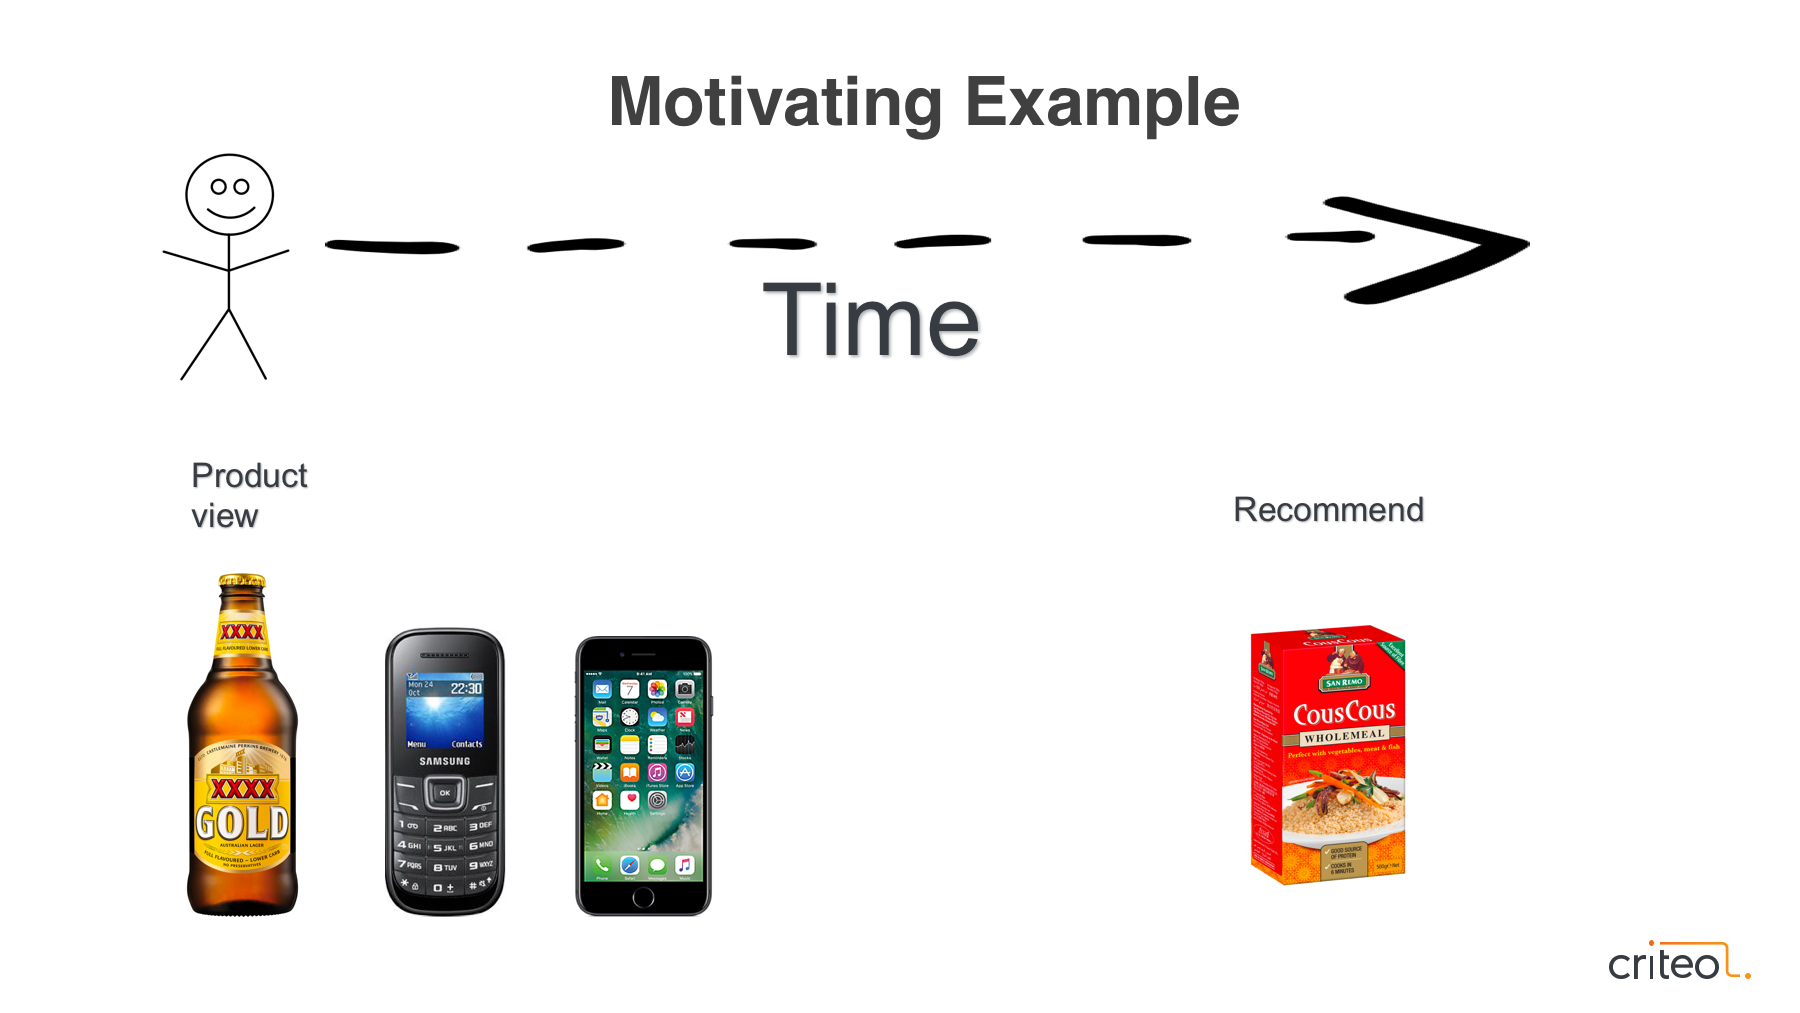
\includegraphics[scale=0.25]{images/mot_ex3.png}
       \centering
       \label{motex1}
   \end{figure}

   \[
   P(C_4=1|A_4={\rm couscous} , V_1 = {\rm beer}, V_2 = {\rm phone ~ A}, V_3 = {\rm phone ~ B}) 
   \]

   
 \end{frame}


 \begin{frame}
  \frametitle{The Real Reco Problem}
 
 
   \begin{figure}[h!]
     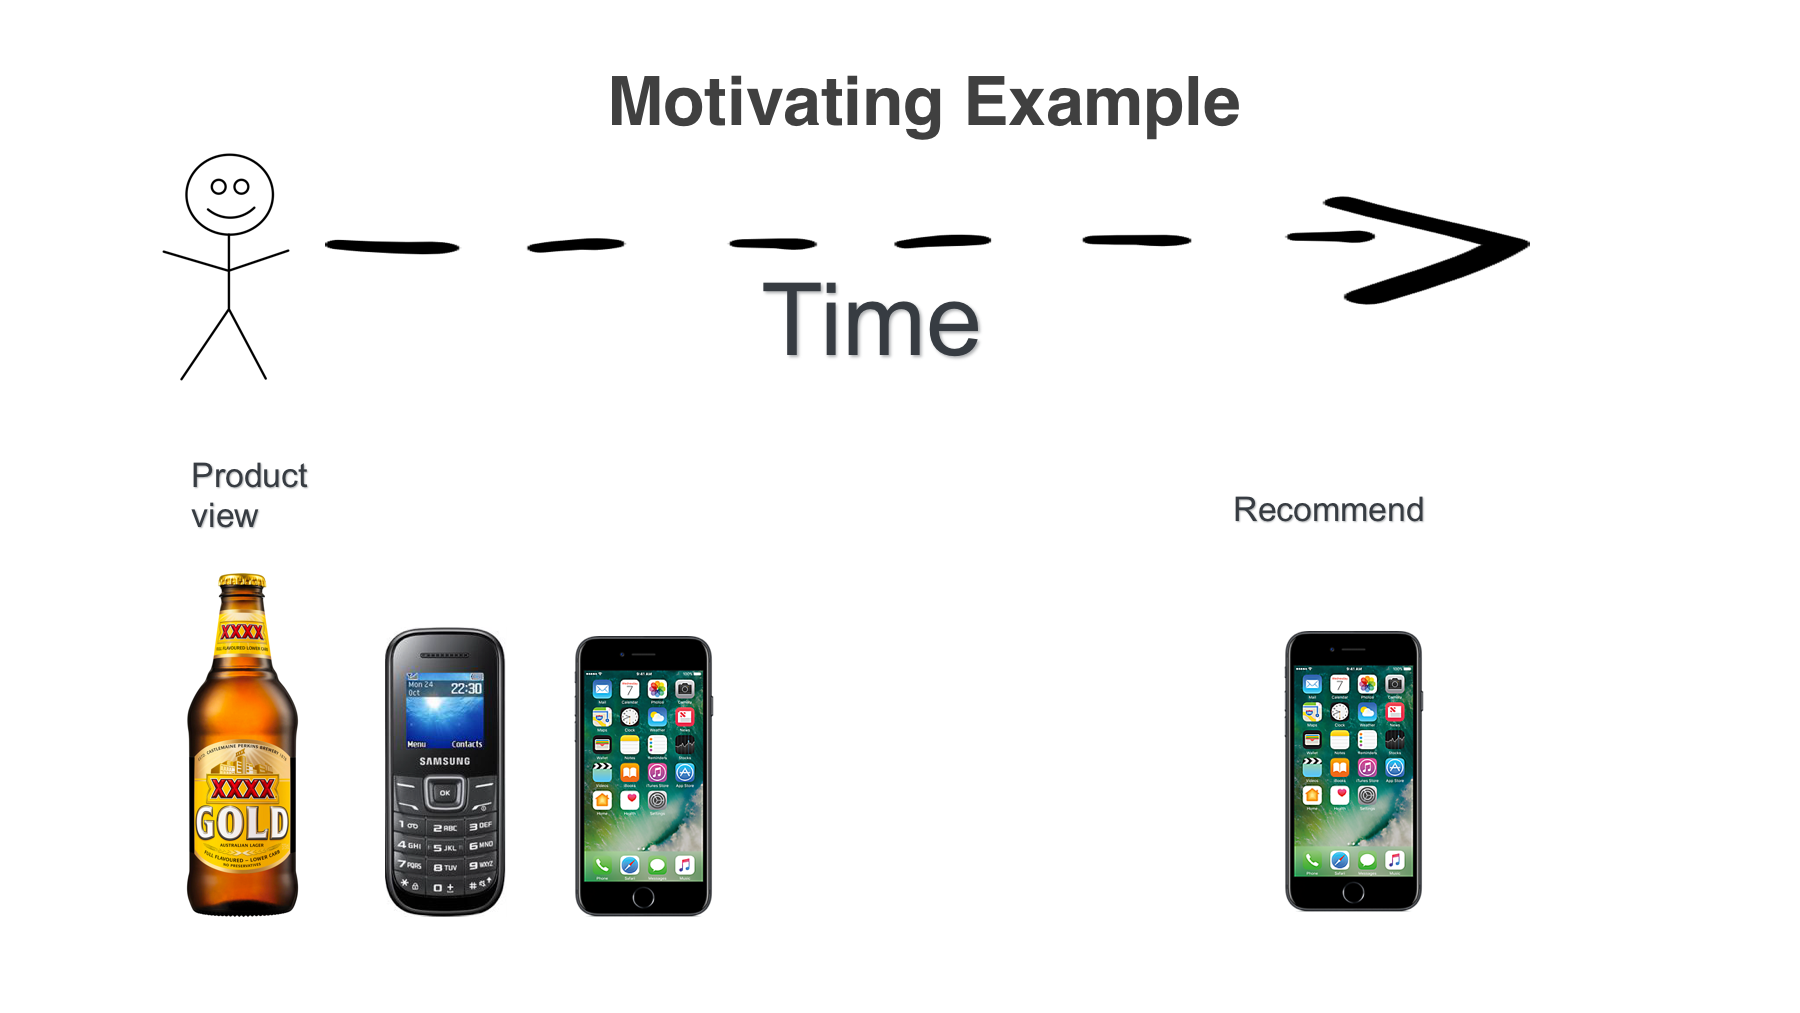
\includegraphics[scale=0.25]{images/mot_ex2.png}
       \centering
       \label{motex1}
   \end{figure}

   \[
   P(C_4=1|A_4={\rm phone ~ B} , V_1 = {\rm beer}, V_2 = {\rm phone ~ A}, V_3 = {\rm phone ~ B}) 
   \]

 \end{frame}


 \begin{frame}
  \frametitle{The Real Reco Problem}
 
 
   \begin{figure}[h!]
     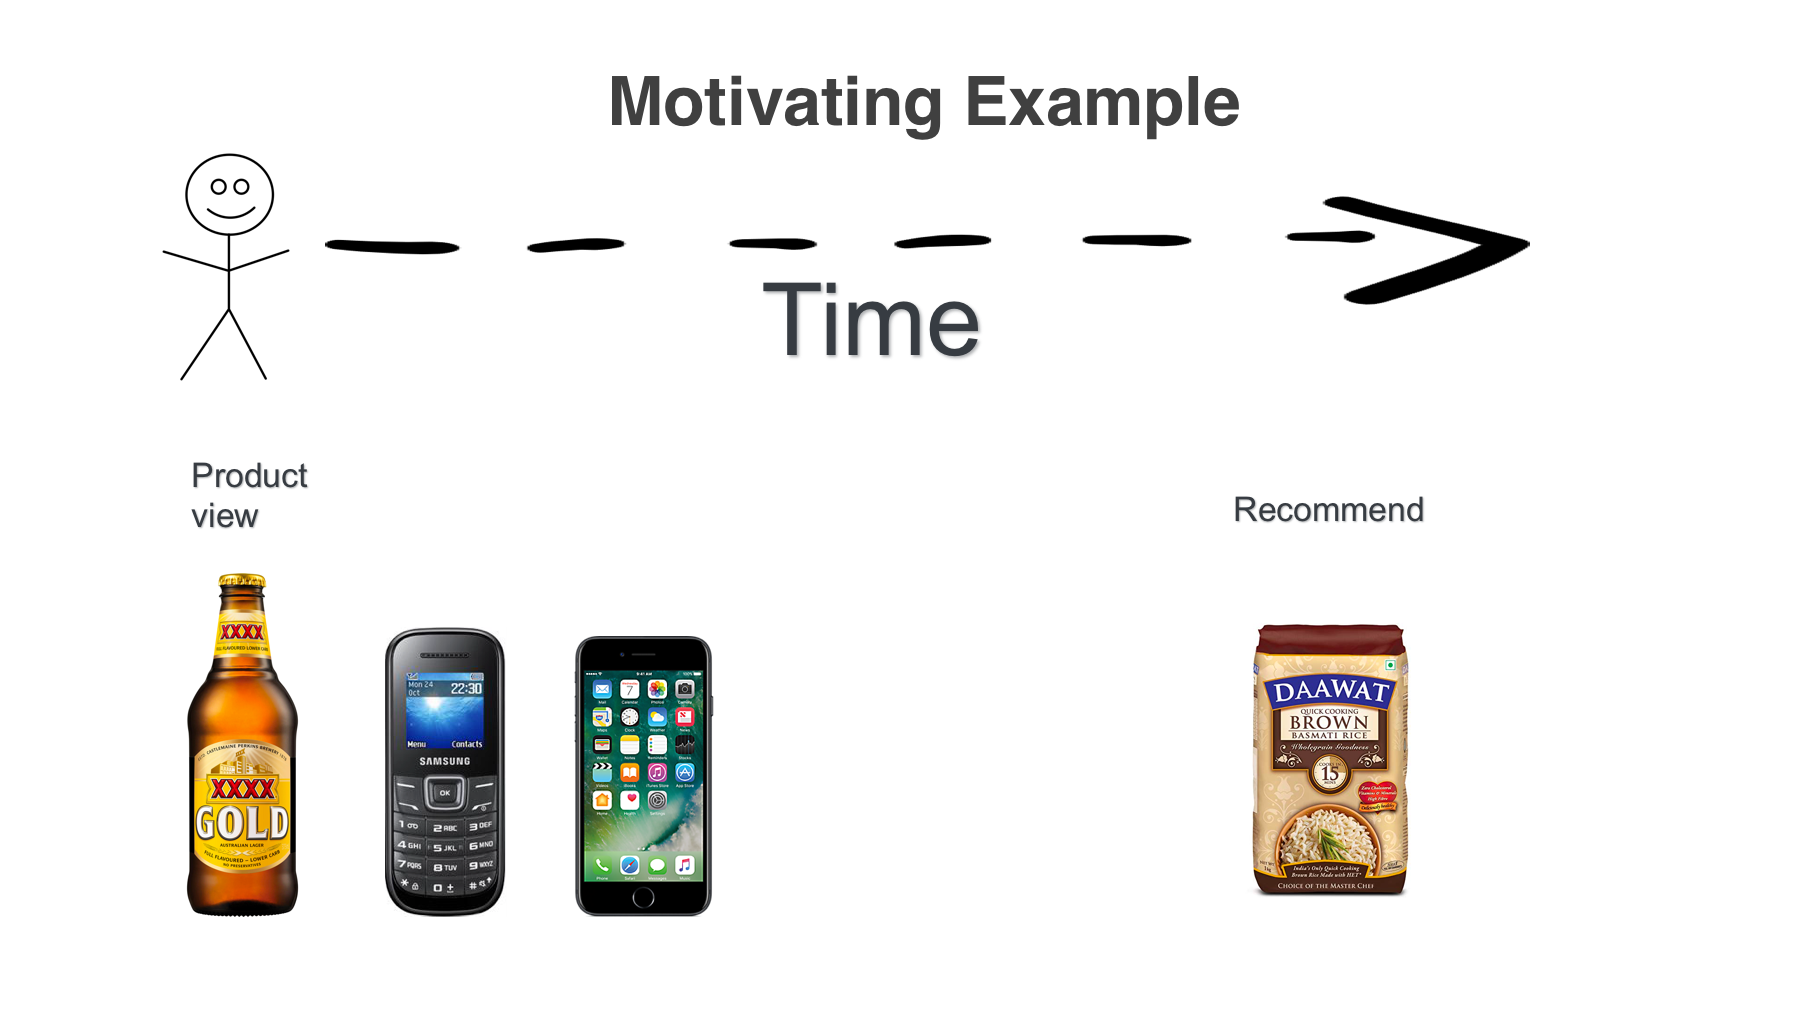
\includegraphics[scale=0.25]{images/mot_ex4.png}
       \centering
       \label{motex1}
   \end{figure}

   \[
   P(C_4=1|A_4={\rm rice},  V_1 = {\rm beer}, V_2 = {\rm phone ~ A}, V_3 = {\rm phone ~ B}) 
   \]
   

 \end{frame}


 \begin{frame}
  \frametitle{What we have, and what we want:}

Our model:
  \begin{tabular}{r l}
    $P(V_4={\rm phone ~ A} |V_1 = {\rm beer}, V_2 = {\rm phone ~ A}, V_3 = {\rm phone ~ A} )$ &= $0.27$ \\
    $P(V_4={\rm phone ~ B} |V_1 = {\rm beer}, V_2 = {\rm phone ~ A}, V_3 = {\rm phone ~ A} )$ &= $0.28$ \\
    $P(V_4={\rm rice} |V_1 = {\rm beer}, V_2 = {\rm phone ~ A}, V_3 = {\rm phone ~ A} )$ &= $.12$ \\
    $P(V_4={\rm couscous} |V_1 = {\rm beer}, V_2 = {\rm phone ~ A}, V_3 = {\rm phone ~ A} )$ &= $.14$ \\
    $P(V_4={\rm beer} |V_1 = {\rm beer}, V_2 = {\rm phone ~ A}, V_3 = {\rm phone ~ A} )$ &= $0.19$ \\
  \end{tabular}

\vspace{1mm}


\pause
Which is a vector of size $P$ that sums to 1.

\vspace{2mm}

We want: \pause

\vspace{1mm}


  \begin{tabular}{r r}
    $P(C_4=1| A_4={\rm phone ~ A}, V_1 = {\rm beer}, V_2 = {\rm phone ~ A}, V_3 = {\rm phone ~ A} )$ &= $?$ \\
    $P(C_4=1| A_4={\rm phone ~ B}, V_1 = {\rm beer}, V_2 = {\rm phone ~ A}, V_3 = {\rm phone ~ A} )$ &= $?$ \\
    $P(C_4=1| A_4={\rm rice}, V_1 = {\rm beer}, V_2 = {\rm phone ~ A}, V_3 = {\rm phone ~ A} )$ &= $?$ \\
    $P(C_4=1| A_4={\rm couscous}, V_1 = {\rm beer}, V_2 = {\rm phone ~ A}, V_3 = {\rm phone ~ A} )$ &= $?$ \\
    $P(C_4=1| A_4={\rm beer}, V_1 = {\rm beer}, V_2 = {\rm phone ~ A}, V_3 = {\rm phone ~ A} )$ &= $?$ \\
  \end{tabular}

\pause
Which is a vector of size $P$ where each entry is between $0$ and $1$.    

 \end{frame}


 \begin{frame}
  \frametitle{An implicit assumption:}

Our model predicts:
  \begin{tabular}{r l}
    $P(V_4={\rm phone ~ A} |V_1 = {\rm beer}, V_2 = {\rm phone ~ A}, V_3 = {\rm phone ~ A} )$ &= $0.27$ \\
    $P(V_4={\rm phone ~ B} |V_1 = {\rm beer}, V_2 = {\rm phone ~ A}, V_3 = {\rm phone ~ A} )$ &= $0.28$ \\
    $P(V_4={\rm rice} |V_1 = {\rm beer}, V_2 = {\rm phone ~ A}, V_3 = {\rm phone ~ A} )$ &= $.12$ \\
    $P(V_4={\rm couscous} |V_1 = {\rm beer}, V_2 = {\rm phone ~ A}, V_3 = {\rm phone ~ A} )$ &= $.14$ \\
    $P(V_4={\rm beer} |V_1 = {\rm beer}, V_2 = {\rm phone ~ A}, V_3 = {\rm phone ~ A} )$ &= $0.19$ \\
  \end{tabular}

So let's recommend phone B, it has the highest next item probability.

\end{frame}

 \begin{frame}
  \frametitle{An implicit assumption:}
If: \pause

\[
P(V_n=a|V_1=v_1..V_{n-1}=v_{n-1}) > P(V_n=b|V_1=v_1..V_{n-1}=v_{n-1})
\]    

\pause
Assume:

\begin{align*}
P(C_n=1|&A_n=a,V_1=v_1..V_{n-1}=v_{n-1}) \\
&> P(C_n=1|A_n=b,V_1=v_1..V_{n-1}=v_{n-1})
\end{align*}

\pause
Vast amounts of academic Reco work assumes this implicitly!

 \end{frame}


 \begin{frame}
  \frametitle{The assumption is testable}

Our model predicts:
  \begin{tabular}{r l}
    $P(V_4={\rm phone ~ A} |V_1 = {\rm beer}, V_2 = {\rm phone ~ A}, V_3 = {\rm phone ~ A} )$ &= $0.27$ \\
    $P(V_4={\rm phone ~ B} |V_1 = {\rm beer}, V_2 = {\rm phone ~ A}, V_3 = {\rm phone ~ A} )$ &= $0.28$ \\
    $P(V_4={\rm rice} |V_1 = {\rm beer}, V_2 = {\rm phone ~ A}, V_3 = {\rm phone ~ A} )$ &= $.12$ \\
    $P(V_4={\rm couscous} |V_1 = {\rm beer}, V_2 = {\rm phone ~ A}, V_3 = {\rm phone ~ A} )$ &= $.14$ \\
    $P(V_4={\rm beer} |V_1 = {\rm beer}, V_2 = {\rm phone ~ A}, V_3 = {\rm phone ~ A} )$ &= $0.19$ \\
  \end{tabular}

So let's recommend phone B, it has the highest next item
probability. \pause - but we will also sometimes choose other actions
with a small probability, so we can check if these items have lower
click through rates.



\end{frame}

 \begin{frame}
  
   \begin{figure}[h!]
     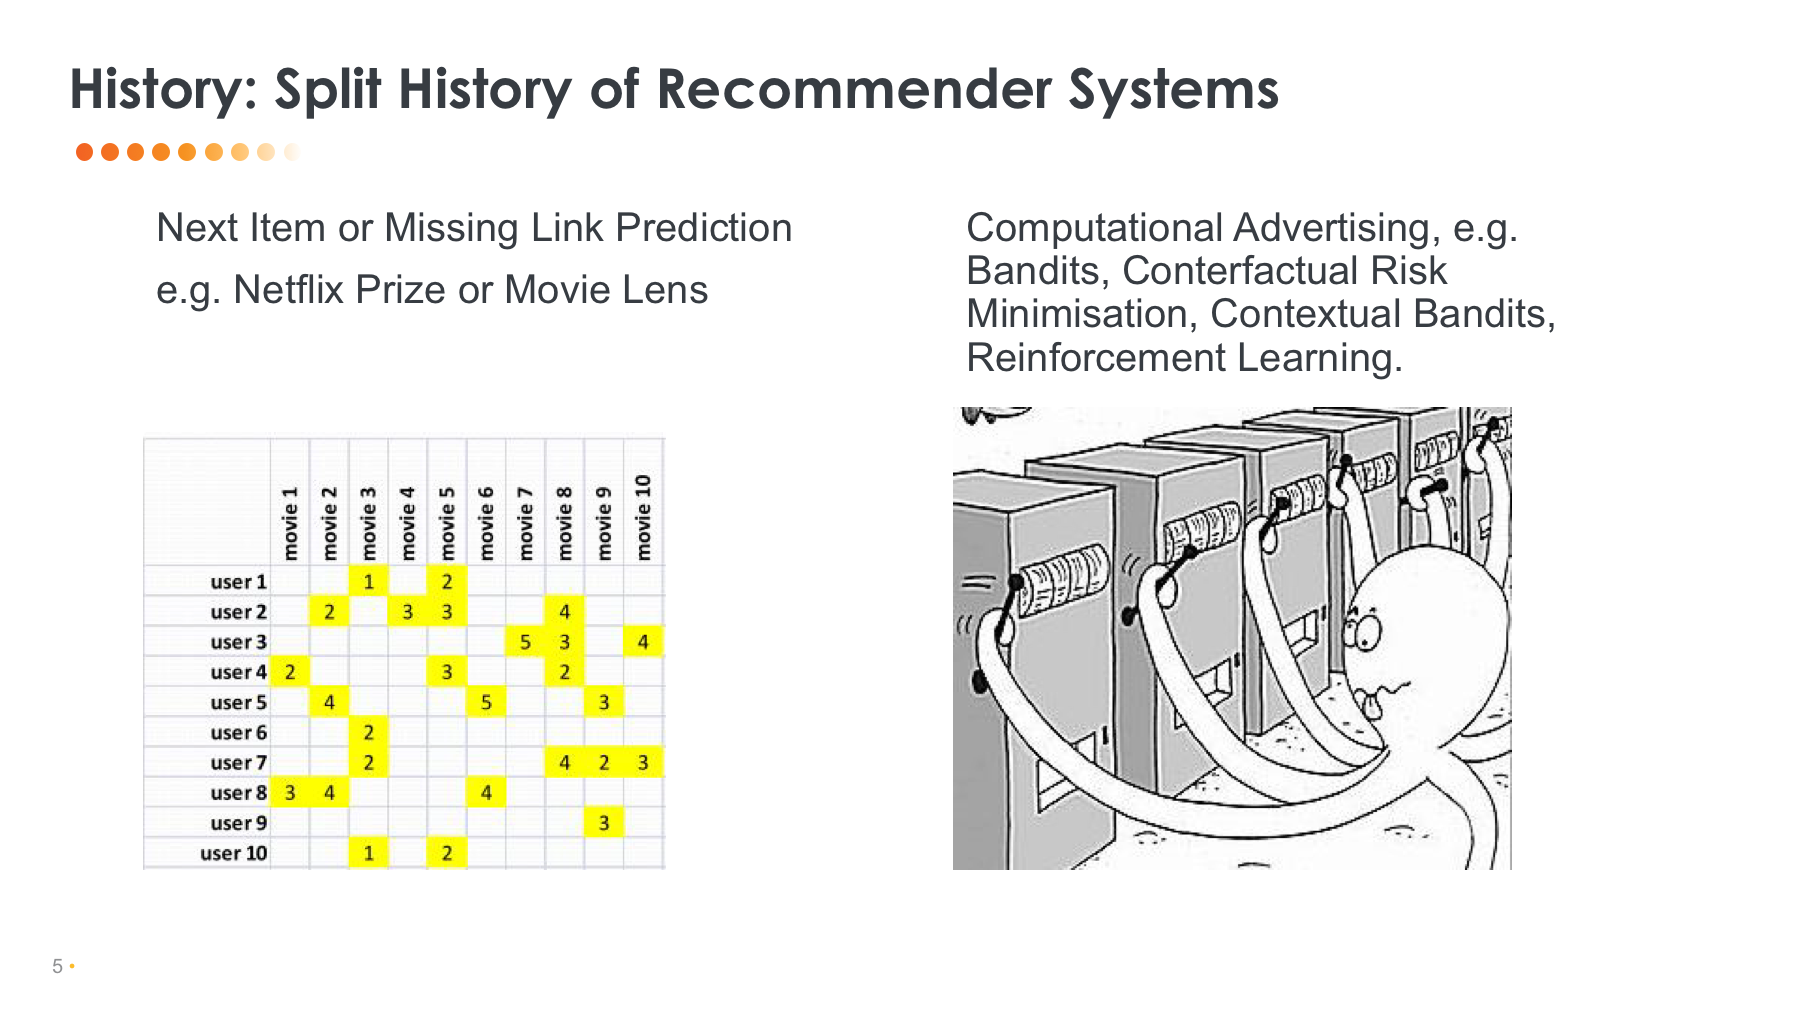
\includegraphics[scale=0.34]{images/octo.png}
       \centering
       \label{motex1}
   \end{figure}
   

 \end{frame}


 \begin{frame}
  \frametitle{Classic RecSys Datasets: Are they logs of recommender systems?}

  \begin{itemize}
    \item MovieLens: \pause no, explicit feedback of movie ratings \pause
    \item Netflix Prize: \pause no, explicit feedback of movie ratings \pause
    \item Yoochoose (RecSys 15): \pause no, implicit session based behavior \pause
    \item 30 Music: \pause no, implicit session based behavior \pause
    \item Yahoo News Feed Dataset \pause yes!
    \item Criteo Dataset for counterfactual evaluation of RecSys algorithms: \pause yes!
  \end{itemize}

  \pause
  The Criteo Dataset shows a log of recommendations and if they were successful in getting users to click.  
\end{frame}



\begin{frame}
  \frametitle{Classic RecSys Evaluation Metrics: Do they evaluate the quality of recommendation?}

  \begin{itemize}
    \item Recall@K, Precision@K, HR@K:  \pause How often is an item in the top k \pause no, evaluates next item prediction \pause
    \item DCG:   \pause Are we assigning high score to an item \pause no, evaluates next item prediction \pause
    \item Log likelihood: \pause  unclear, but ususally next item prediction \pause
    \item Inverse Propensity Score estimate of click through rate: \pause to be explained later. \pause yes! (although it is often noisy) \pause
    \item AB Test: \pause i.e. run a randomized control trial live\pause yes, but the academic literature has no access to this 
  \end{itemize}

  \pause
If the dataset does not contain a log of recommendations and if they were successful, you cannot compute metrics of the recommendation quality.
\end{frame}



\begin{frame}
  \frametitle{Offline evaluation that predicts an AB test result}

Imagine we have a new recommendation stratergy $\pi_t(A_{n}=a_n|V_1=v_1,...,V_n=v_{n-1})$, can we
predict how well it will perform if we deploy it?  We collect logs
from a different policy: $\pi_0(A_{n}=a_n|V_1=v_1,...,V_n=v_{n-1})$

\pause

Let's examine some hypothetical logs... 

 \end{frame}



\begin{frame}
  \frametitle{Offline evaluation IPS}
 
 
   \begin{figure}[h!]
     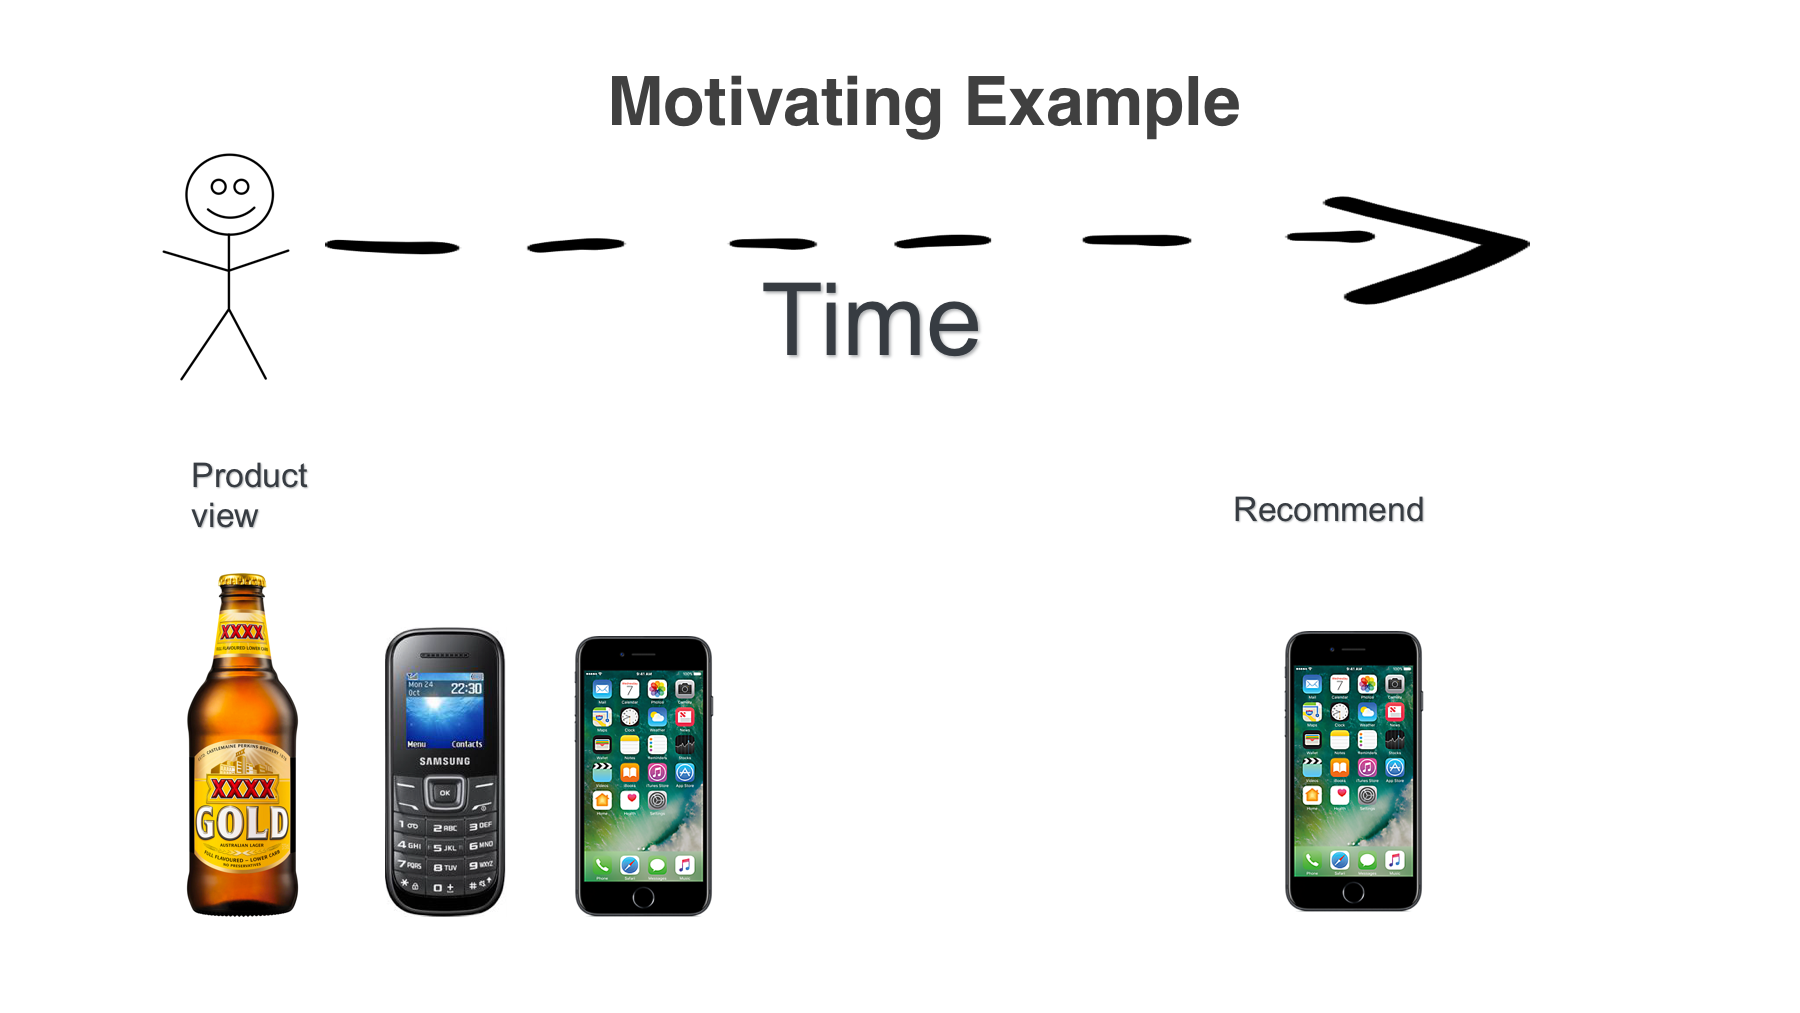
\includegraphics[scale=0.15]{images/mot_ex2.png}
       \centering
       \label{motex1}
   \end{figure}

Imagine the user clicks
\begin{align*}
     \pi_t(A_{4}= {\rm phone ~ B} {\rm }|V_1={\rm beer}, V_2={\rm phone ~ A}, V_3={\rm phone ~ B}) &= 1\\
     \pi_0(A_{4}= {\rm phone ~ B} {\rm }|V_1={\rm beer}, V_2={\rm phone ~ A}, V_3={\rm phone ~ B}) &= 0.8\\
\end{align*}

The new policy will recommend ``phone B'' the $\frac{1}{0.8}=1.25 \times$ as often as the old policy.
   
 \end{frame}




\begin{frame}
  \frametitle{Offline evaluation IPS}
 
  \begin{figure}[h!]
    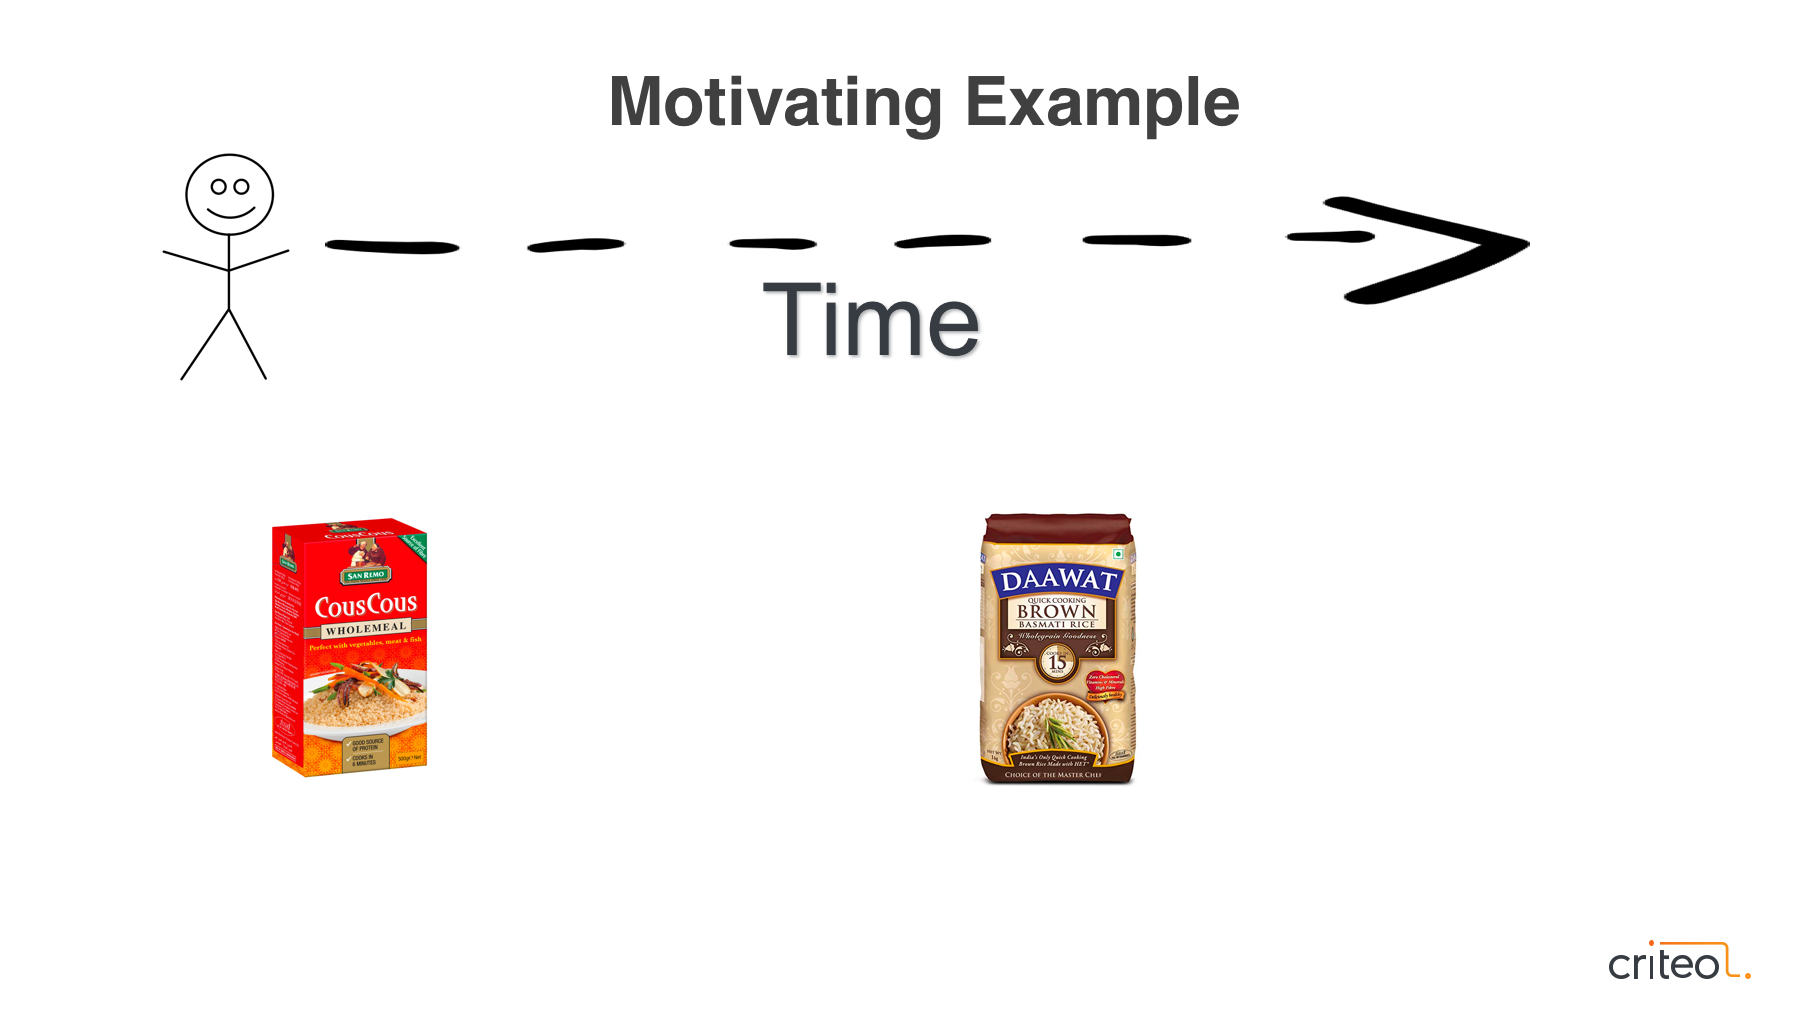
\includegraphics[scale=0.15]{images/rice_cous.png}
      \centering
      \label{motex1}
  \end{figure}


Imagine the user clicks
\begin{align*}
     \pi_t(A_{2}= {\rm rice} {\rm }|V_1={\rm couscous}) &= 1\\
     \pi_0(A_{2}= {\rm rice} {\rm }|V_1={\rm couscous}) &= 0.01\\
\end{align*}

The new policy will recommend ``rice'' the $\frac{1}{0.01}=100 \times$ as often as the old policy.
   
 \end{frame}


\begin{frame}
  \frametitle{Offline evaluation IPS}
 
\[
{\rm CTR ~ estimate} = \frac{1}{N} \sum_n^N \frac{c_n \pi_t(A_n=a_n|V_1=v_1..V_n=v_n)}{\pi_0(A_n=a_n|V_1=v_1..V_n=v_n)}
\]

\pause
We only look at the clicks i.e. $c_n=1$ (otherwise the contribution is $0$).

\pause

When the new policy differs markedly from the old, the weights become
very high (to compensate for the fact that these are rare examples in
your sample).  These rare high values contribute a lot to the variance
of the estimator.


\pause
IPS actually atempts to predict the AB test, but it often has less
than spectacular results...   

 \end{frame}

\begin{frame}
  \frametitle{Real world Reco}

Real world reco is an anonymous hybrid of different methodologies.
Often poor agreement between online and offline metrics are
reported..  \pause why? \pause What does real world reco look like?

\end{frame}

  
\begin{frame}
  \frametitle{Recommendation as Supervised Learning and AB Testing}
 
 
   \begin{figure}[h!]
     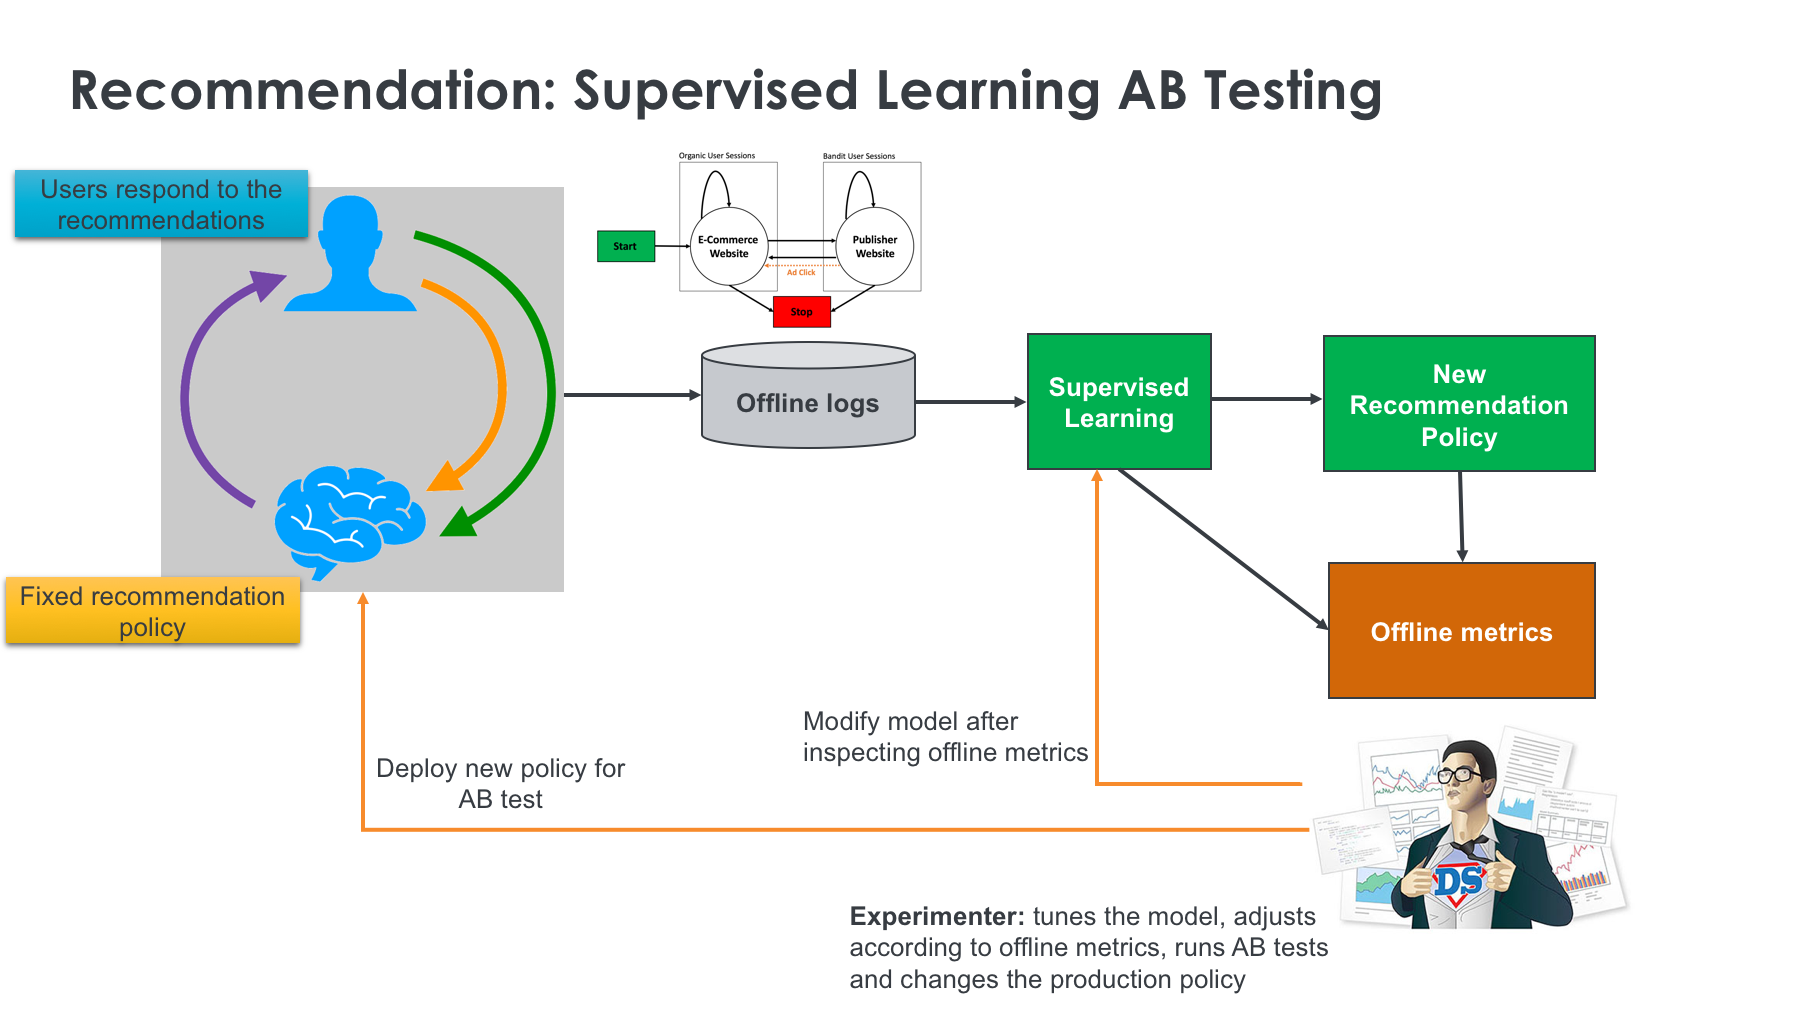
\includegraphics[scale=0.3]{images/recoasabtesting0.png}
       \centering
       \label{motex1}
   \end{figure}
     
 \end{frame}

      


\begin{frame}
\frametitle{Recommendation as Supervised Learning and AB Testing}


 \begin{figure}[h!]
   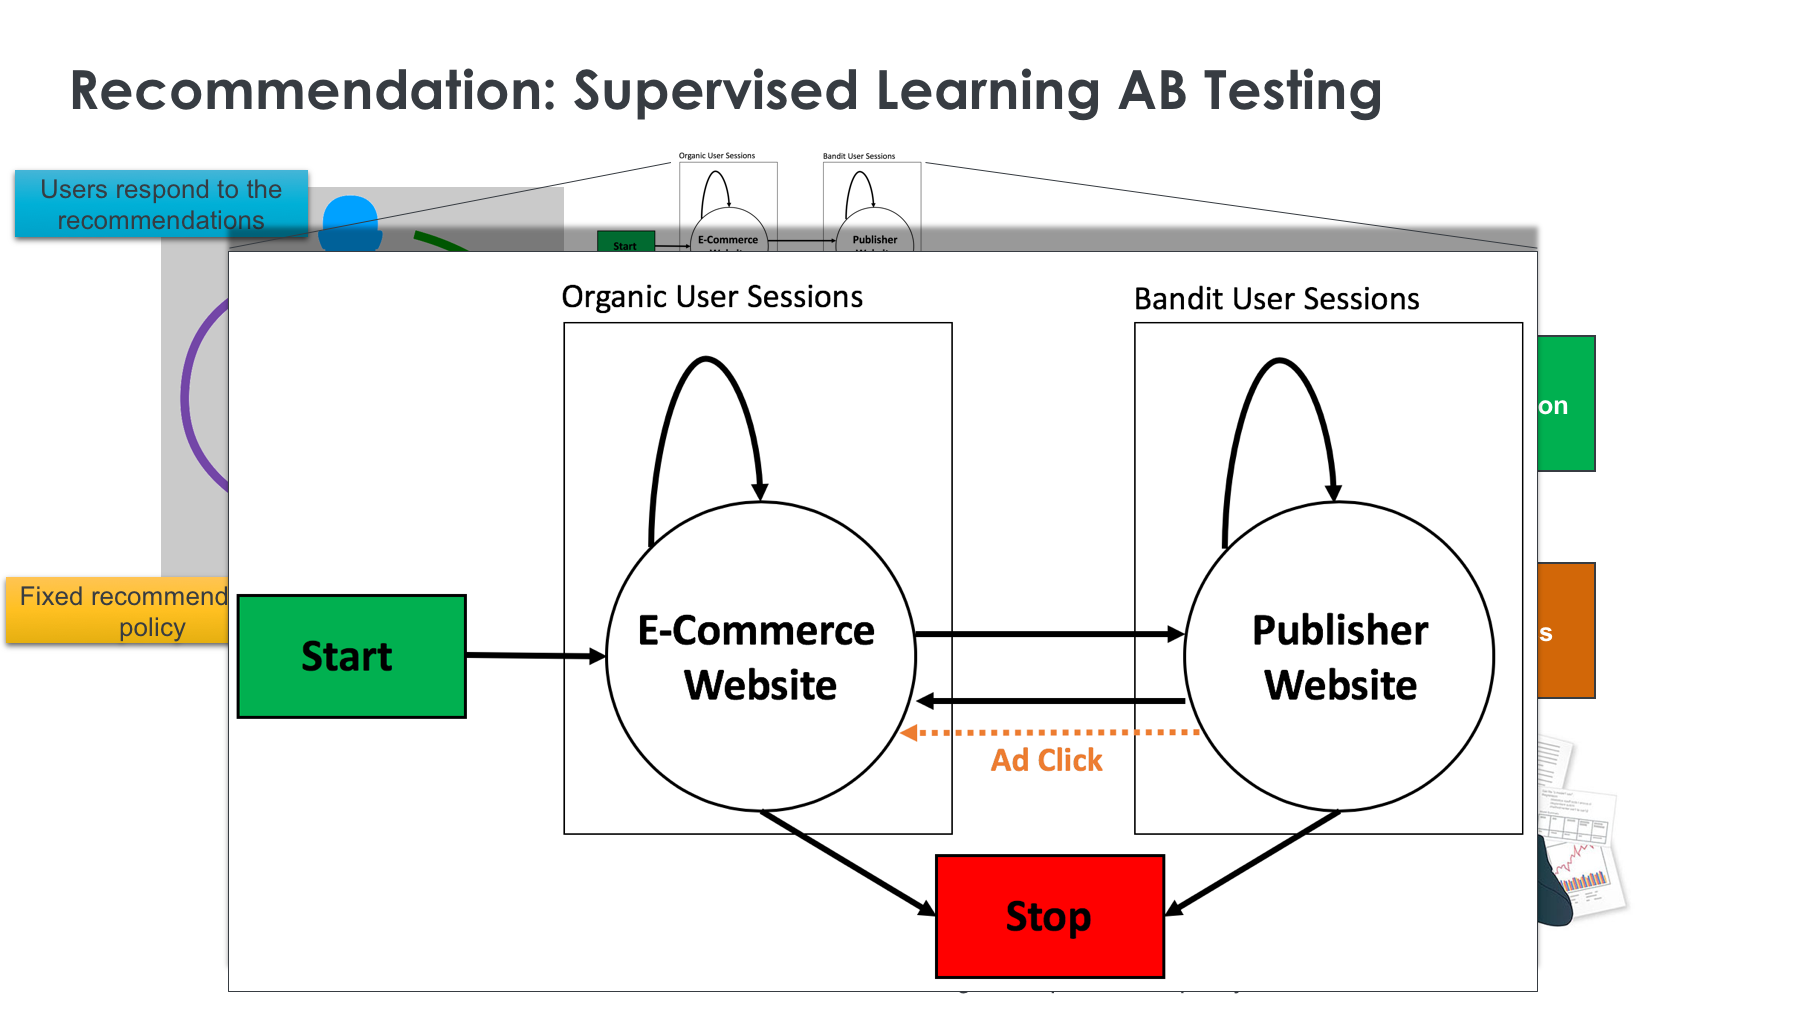
\includegraphics[scale=0.3]{images/recoasabtesting.png}
     \centering
     \label{motex1}
 \end{figure}
   
\end{frame}



\begin{frame}
  \frametitle{Let's take a step back...}
  
  \textbf{How are we improving large-scale Recommender Systems in the Real World}
  
  \begin{itemize}
  \item Learn a supervised model from past user activity
  \item Evaluate offline and decide whether to A/B test
  \item A/B test
  \item If positive and scalable, roll-out
  \item If not, try to understand what happened and try to create a better model of the world using the same past data
  \item Repeat
  \end{itemize}
        
  \end{frame}
  

  
  \begin{frame}
    \frametitle{Supervised learning with the wrong objective}
  
  We are operating under the assumption that the best recommendation policy is in some sense the \textbf{optimal auto-complete of natural user behavior}
  
  \end{frame}
  
  
  \begin{frame}
    \frametitle{Supervised learning with the wrong objective}
  
  From the point of view of business metrics, \textbf{learning to autocomplete behavior is a great initial recommendation policy}, especially when no prior user feedback is available. 
  
  \pause
  \textbf{However}, after a first golden age, where all offline improvements turn into positive A/B tests, the \emph{naive recommendation} optimization objective and the business objective will start to diverge.
  
  \end{frame}
  
  
  \begin{frame}
    \frametitle{Aligning the Recommendation objective with the business}
  
  \begin{itemize}
  \item Of course, we could start incorporating user feedback that we collected while running the initial recommendation policies  
  \item We should be able to continue bringing improvements using feedback that is now aligned with our business metrics (ad CTR, post click sales, dwell time, number of videos watched, ...)
  \end{itemize}
  
  \end{frame}
  
  




 
\begin{frame}
  \frametitle{Modern Recommendation Systems Research}
  
  \textbf{Q: How does the literature on Large Scale Recommendation Systems look right now?}
  
  A: Most of the latest publications are talking about ways of using Deep Learning for Recommendation:
  \begin{itemize}
  \item \textbf{Matrix Factorization extensions:} Word2Vec, Deep and Wide, Neural MF, Node2Vec 
  \item \textbf{Content-based recommendation:} CNNs for Image, Text, Sounds to compute item similarities
  \item \textbf{Next event prediction / user activity modeling:} RNNs, TCNs
  \end{itemize}
  
\end{frame}


\begin{frame}
  \frametitle{Modern Recommendation Systems Research}
  
  \textbf{We see great improvements in offline metrics!}
  
  \begin{itemize}
  \item \textbf{Regression/Classification metrics:} MSE, AUC, NLL
  \item \textbf{Ranking metrics:} MPR, Precision@k, NDCG
  \end{itemize}
  
\end{frame}


\begin{frame}
  \frametitle{What is wrong with this picture?}
  
	\textbf{In the same time, as practitioners, we see difficulties in improving the Real World Recommendation models!}

	Offline - online metrics alignment for recommendation is a recognized problem:
	\begin{itemize}
	\item \textbf{Previous work:} Missing Not At Random (MNAR) framework for Matrix factorization, Bandits Literature
	\item \textbf{New avenues:}  \emph{REVEAL: Offline evaluation for recommender systems Workshop at RecSys 2019} (this September in Copenhagen) \url{https://recsys.acm.org/recsys19/reveal/}
	\end{itemize}
  
\end{frame}


\begin{frame}
  \frametitle{The relationship between Reinforcement Learning and Recommendation}

\begin{itemize}
\item We are doing Reinforcement Learning by hand!
\pause
\item Furthermore, we are trying to do RL using the Supervised Learning Framework
\pause
\item Standard test data sets do not let us explore this aspect of recommender systems
\end{itemize}

\pause
.. but how do you evaluate a reinforcement learning algorithm?
\end{frame}

  



\begin{frame}
  \frametitle{}
 
 
   \begin{figure}[h!]
     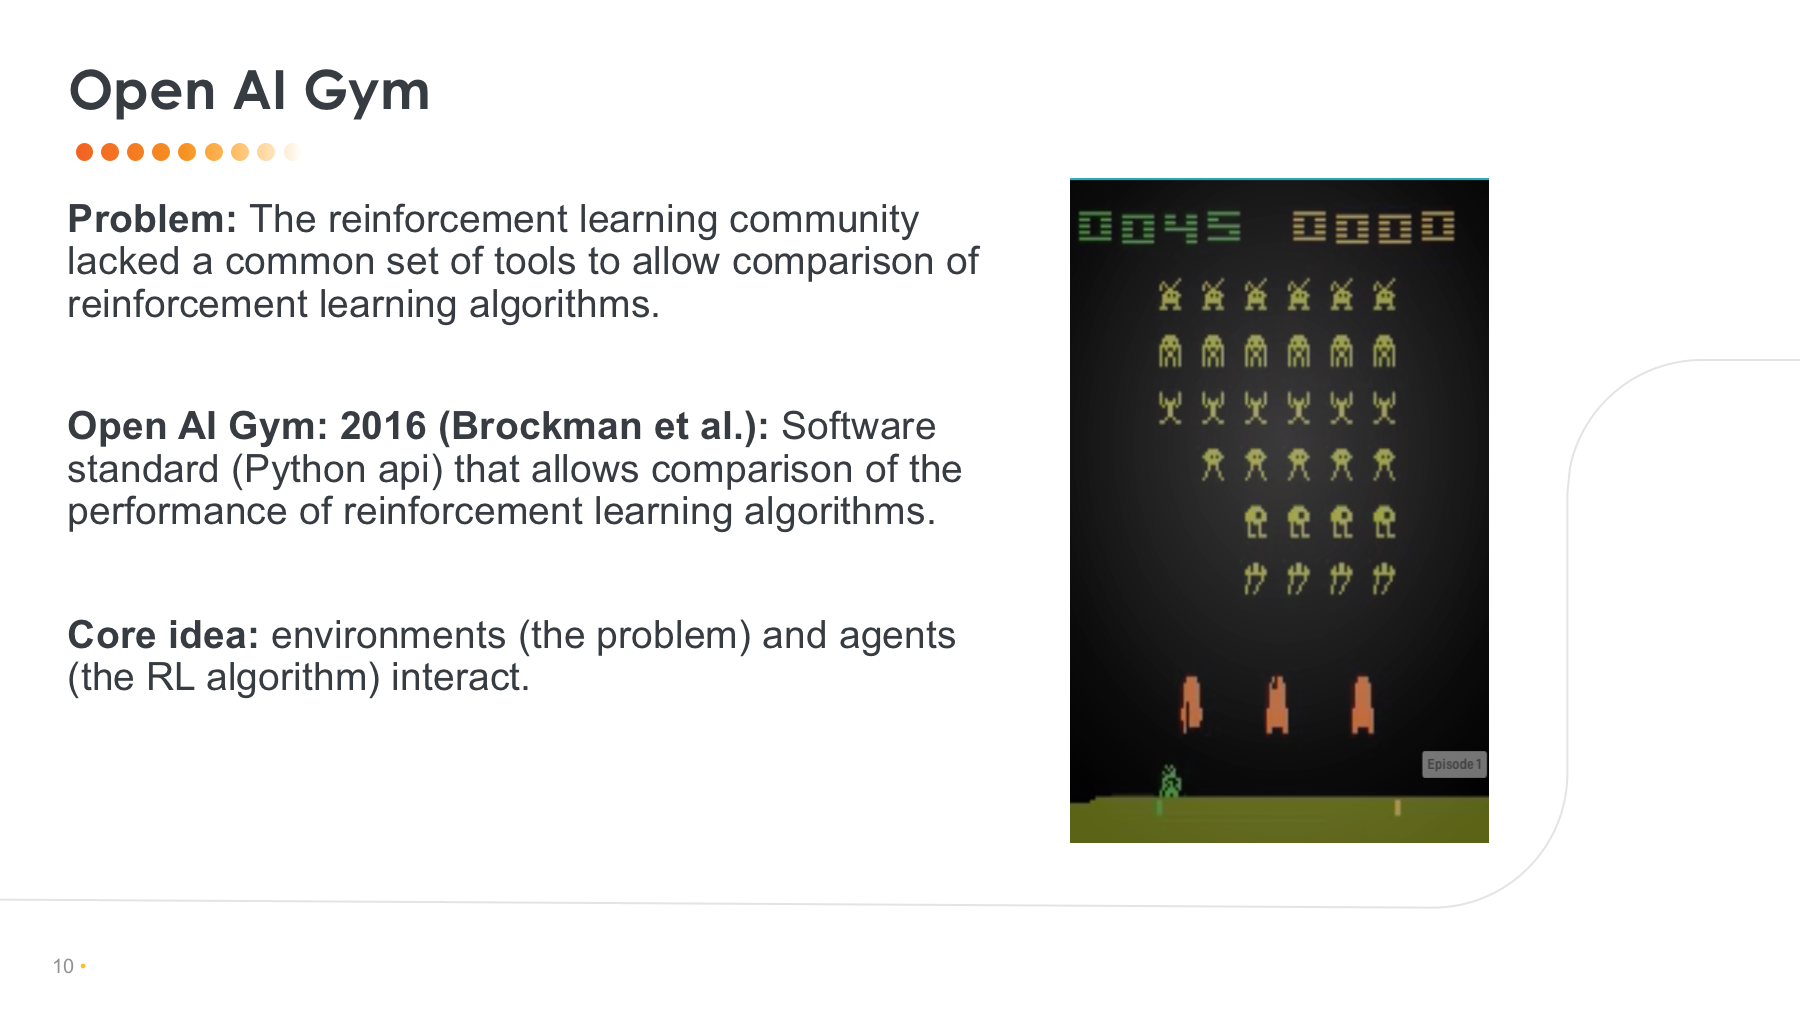
\includegraphics[scale=0.39]{images/openai.png}
       \centering
       \label{motex1}
   \end{figure}
     
 \end{frame}



 \begin{frame}
  \frametitle{}
 
 
   \begin{figure}[h!]
     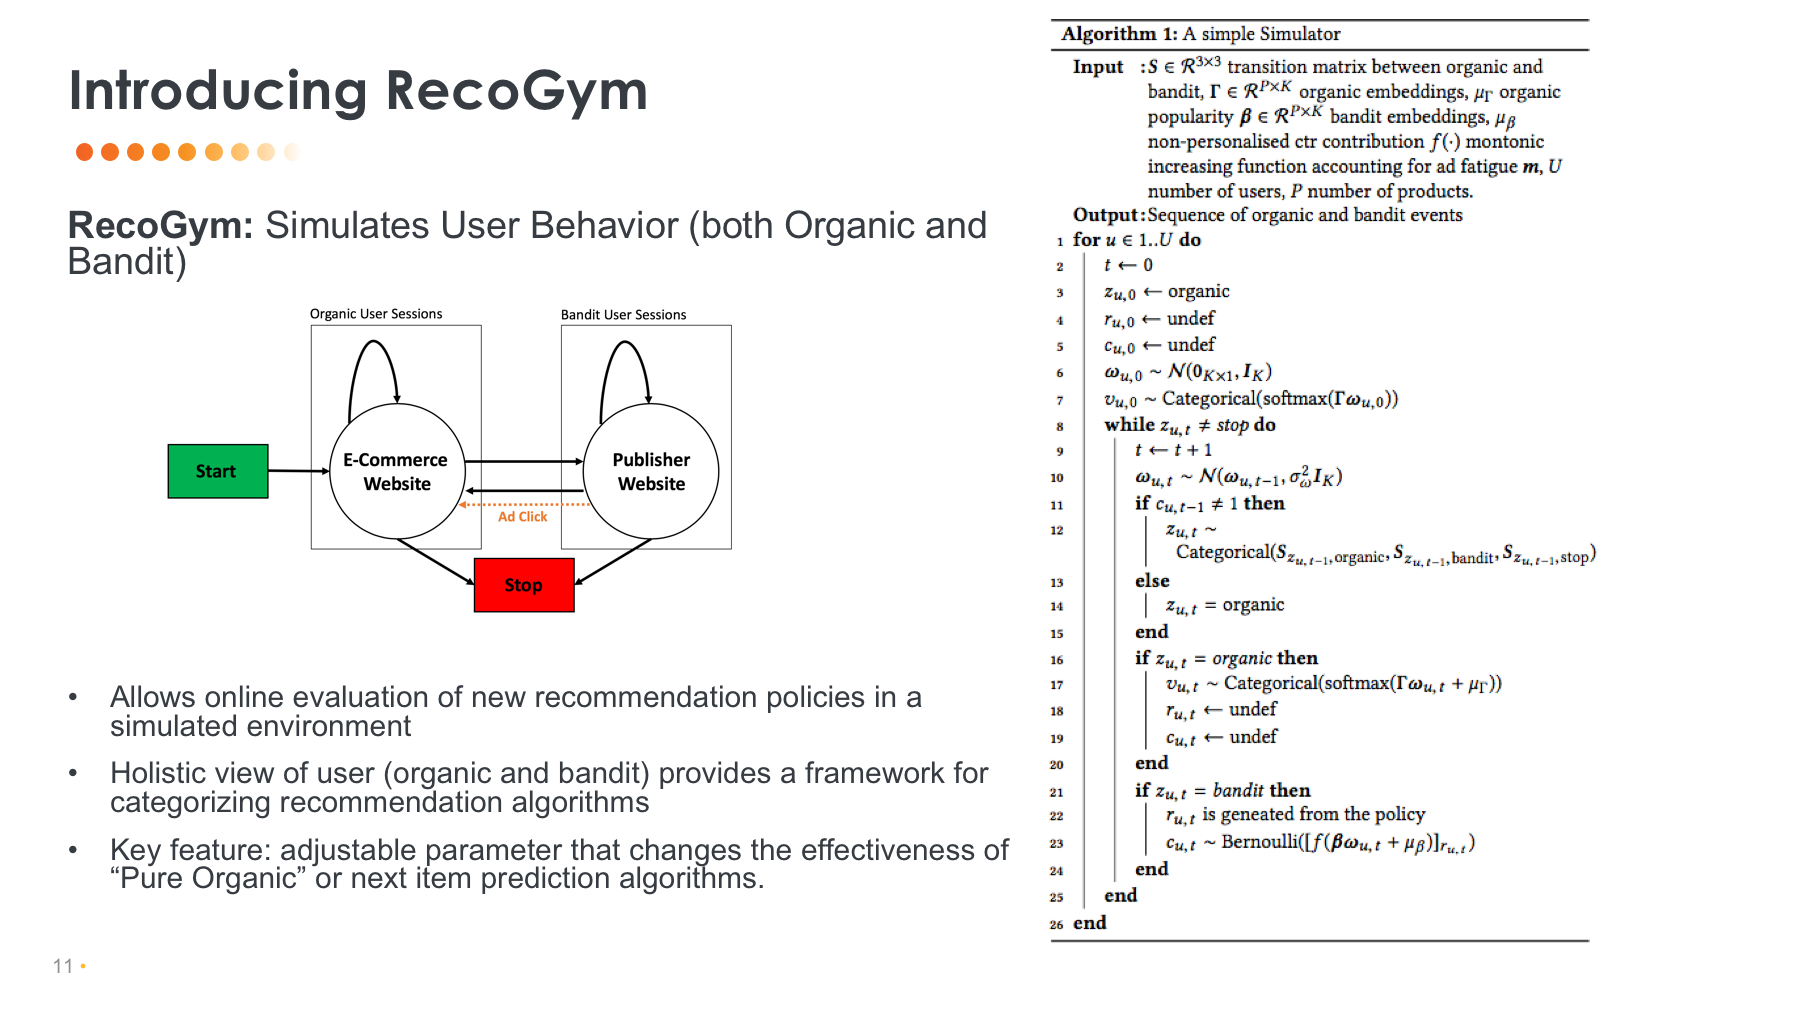
\includegraphics[scale=0.34]{images/recogym1}
       \centering
       \label{motex1}
   \end{figure}
     
 \end{frame}





 \begin{frame}
  \frametitle{}
 
 
   \begin{figure}[h!]
     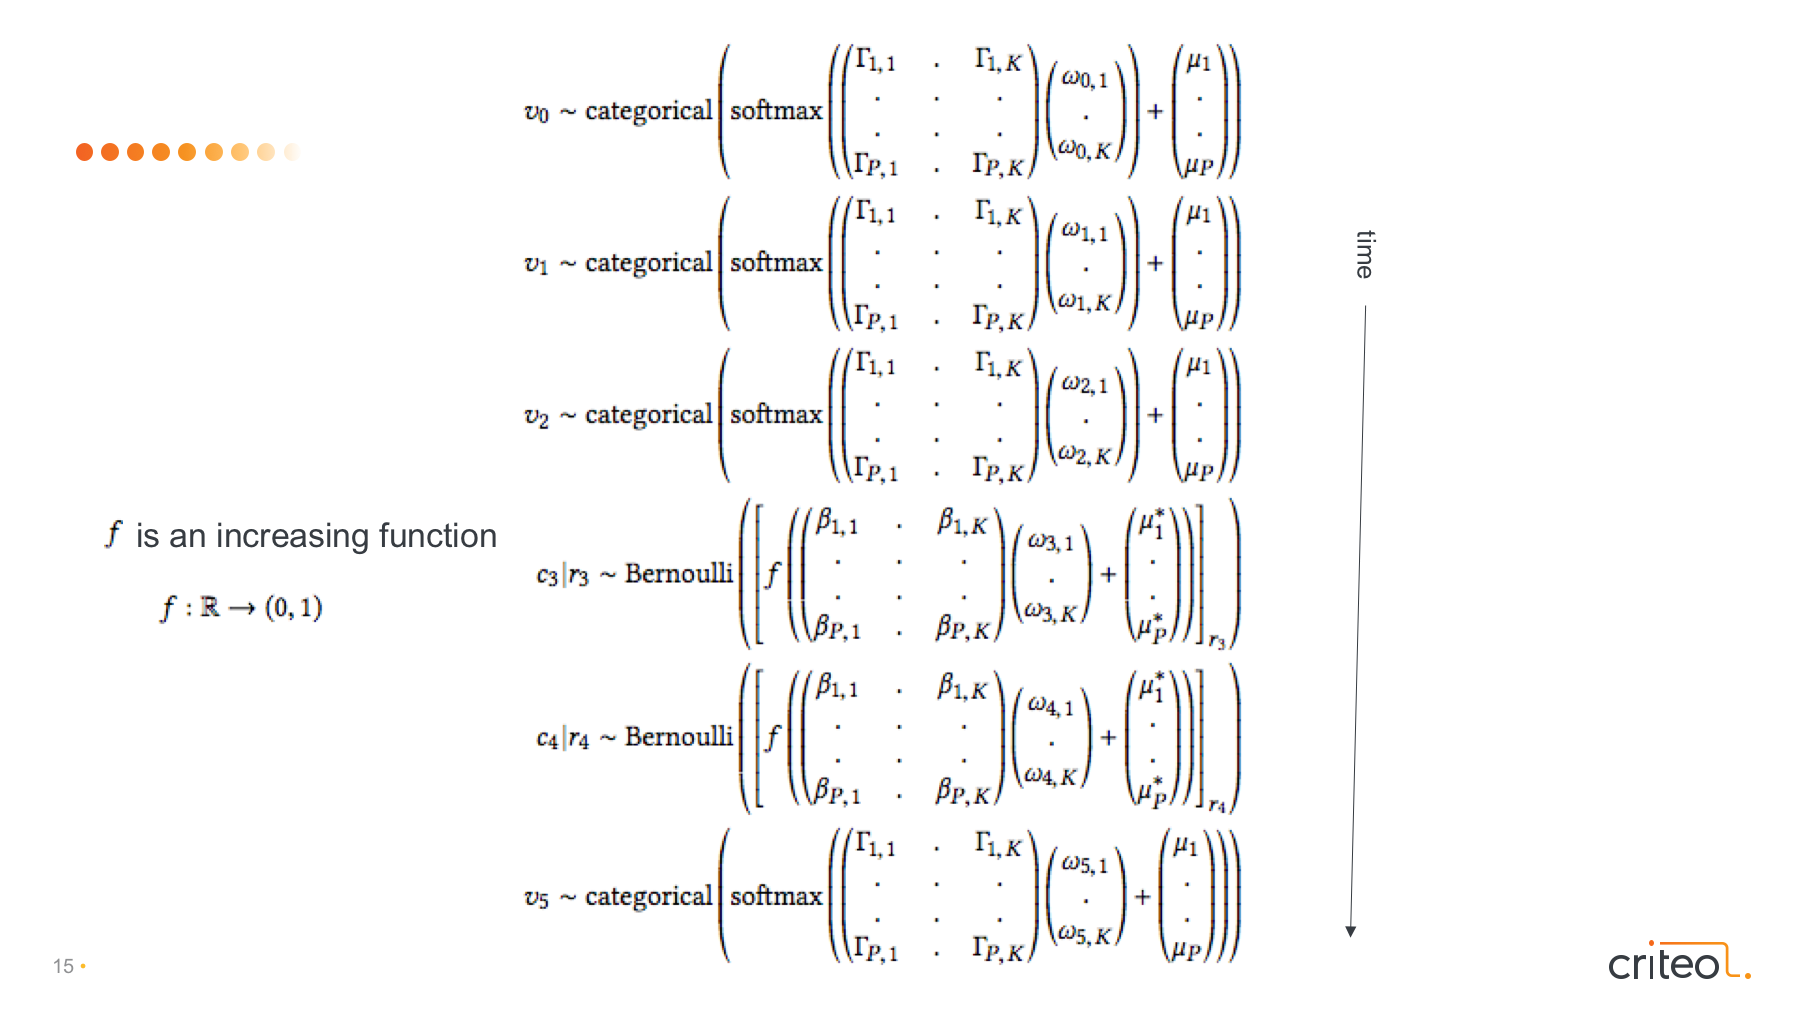
\includegraphics[scale=0.3]{images/recogymsim}
       \centering
       \label{motex1}
   \end{figure}
     
 \end{frame}



 \begin{frame}
  \frametitle{The RecoGym Session}
 
 
   \begin{figure}[h!]
     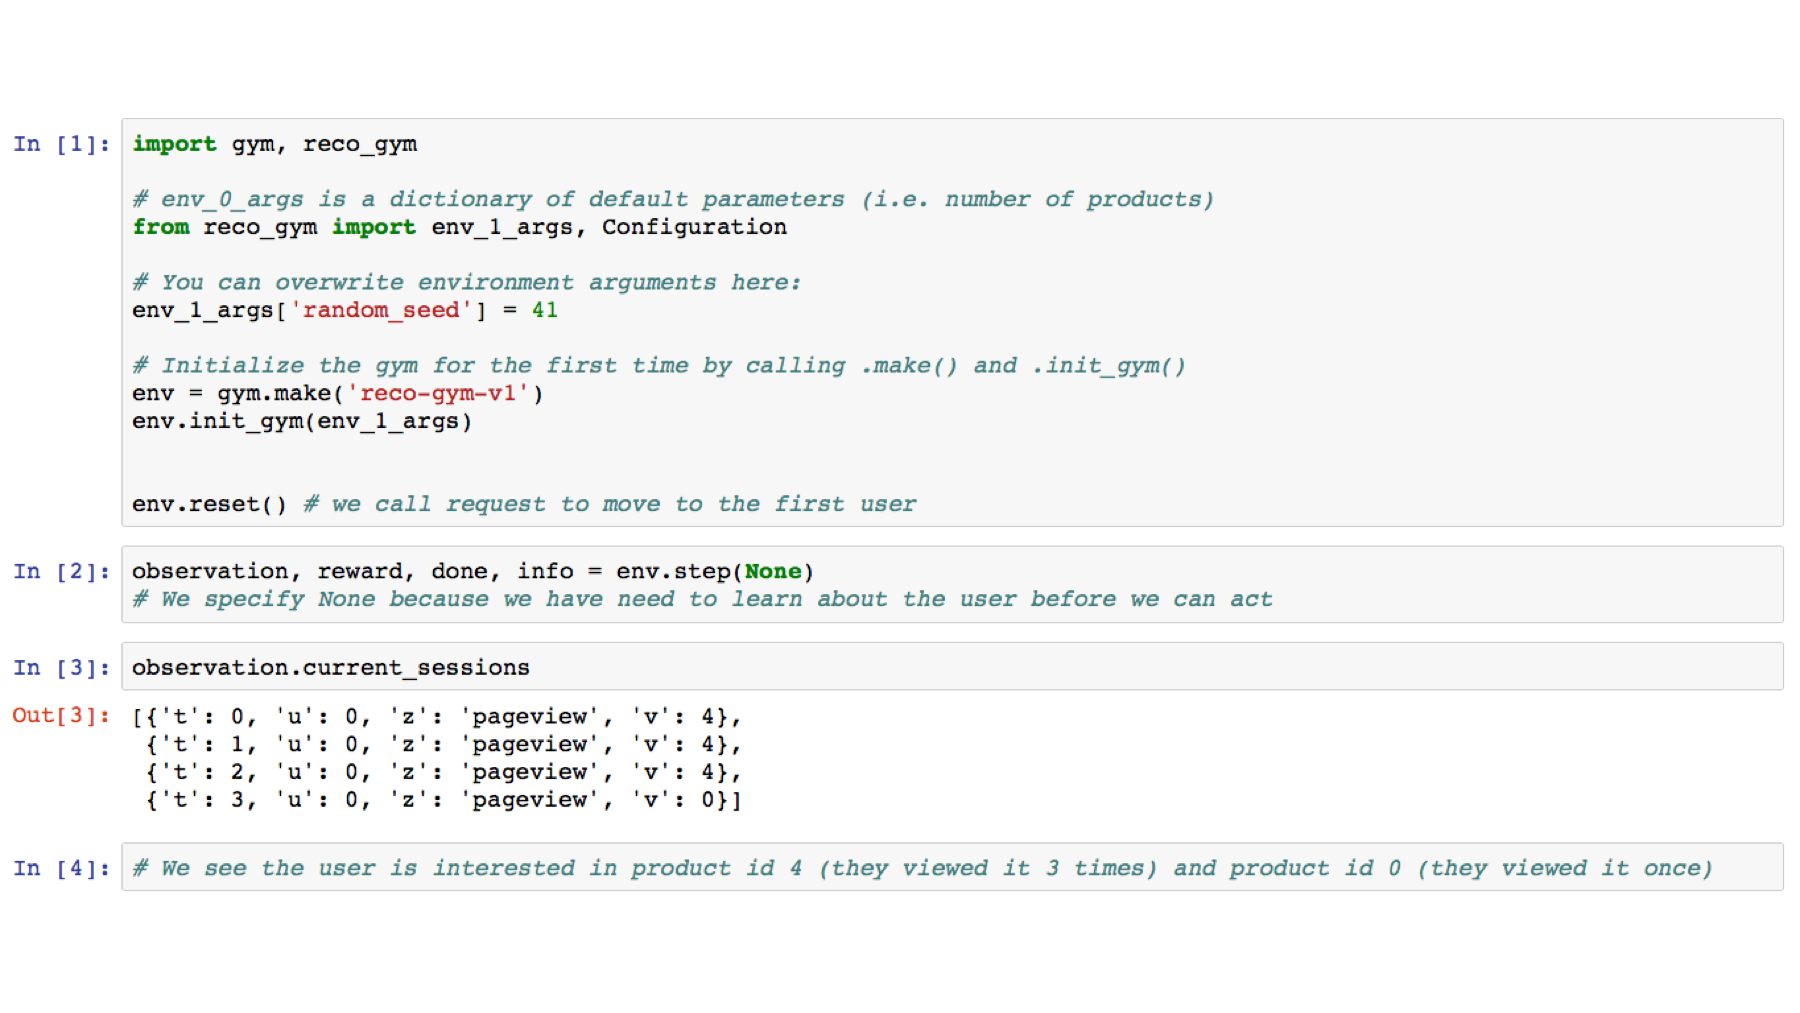
\includegraphics[scale=0.3]{images/reco_gym_sess0.png}
       \centering
       \label{motex1}
   \end{figure}
     
 \end{frame}



 \begin{frame}
  \frametitle{The RecoGym Session}
 
 
   \begin{figure}[h!]
     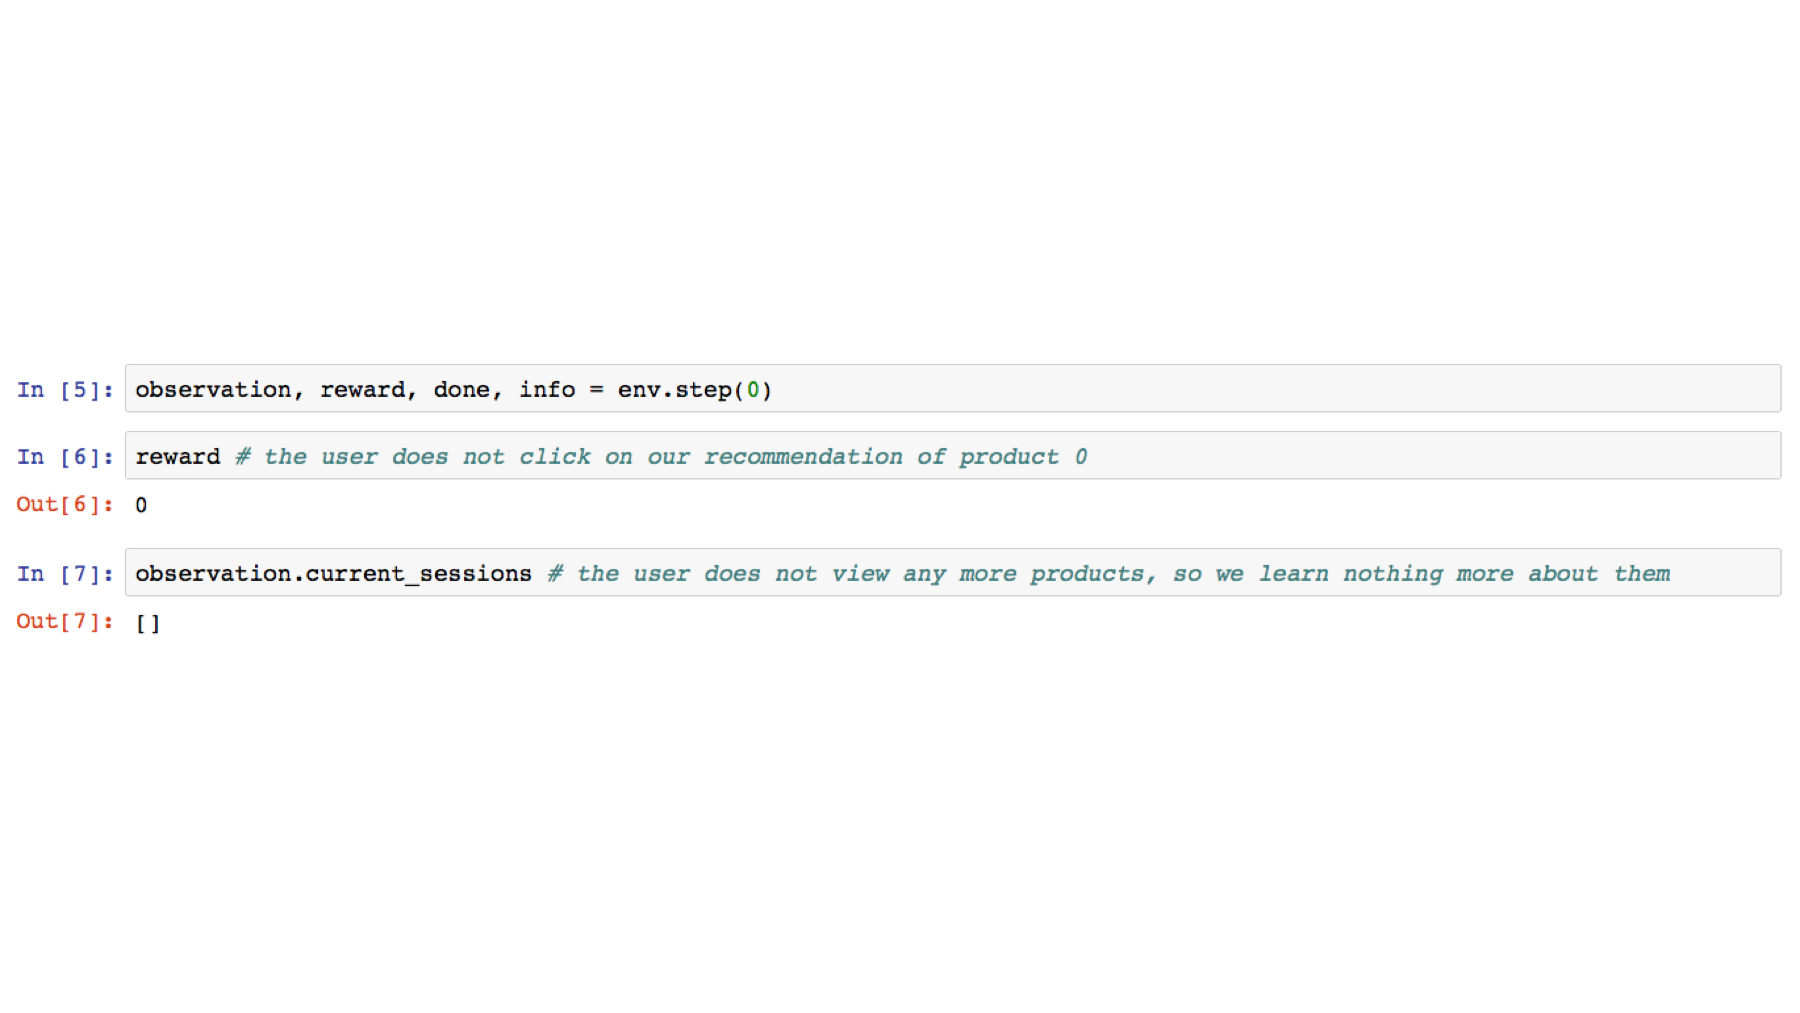
\includegraphics[scale=0.3]{images/reco_gym_sess1.png}
       \centering
       \label{motex1}
   \end{figure}
     
 \end{frame}



 \begin{frame}
  \frametitle{The RecoGym Session}
 
 
   \begin{figure}[h!]
     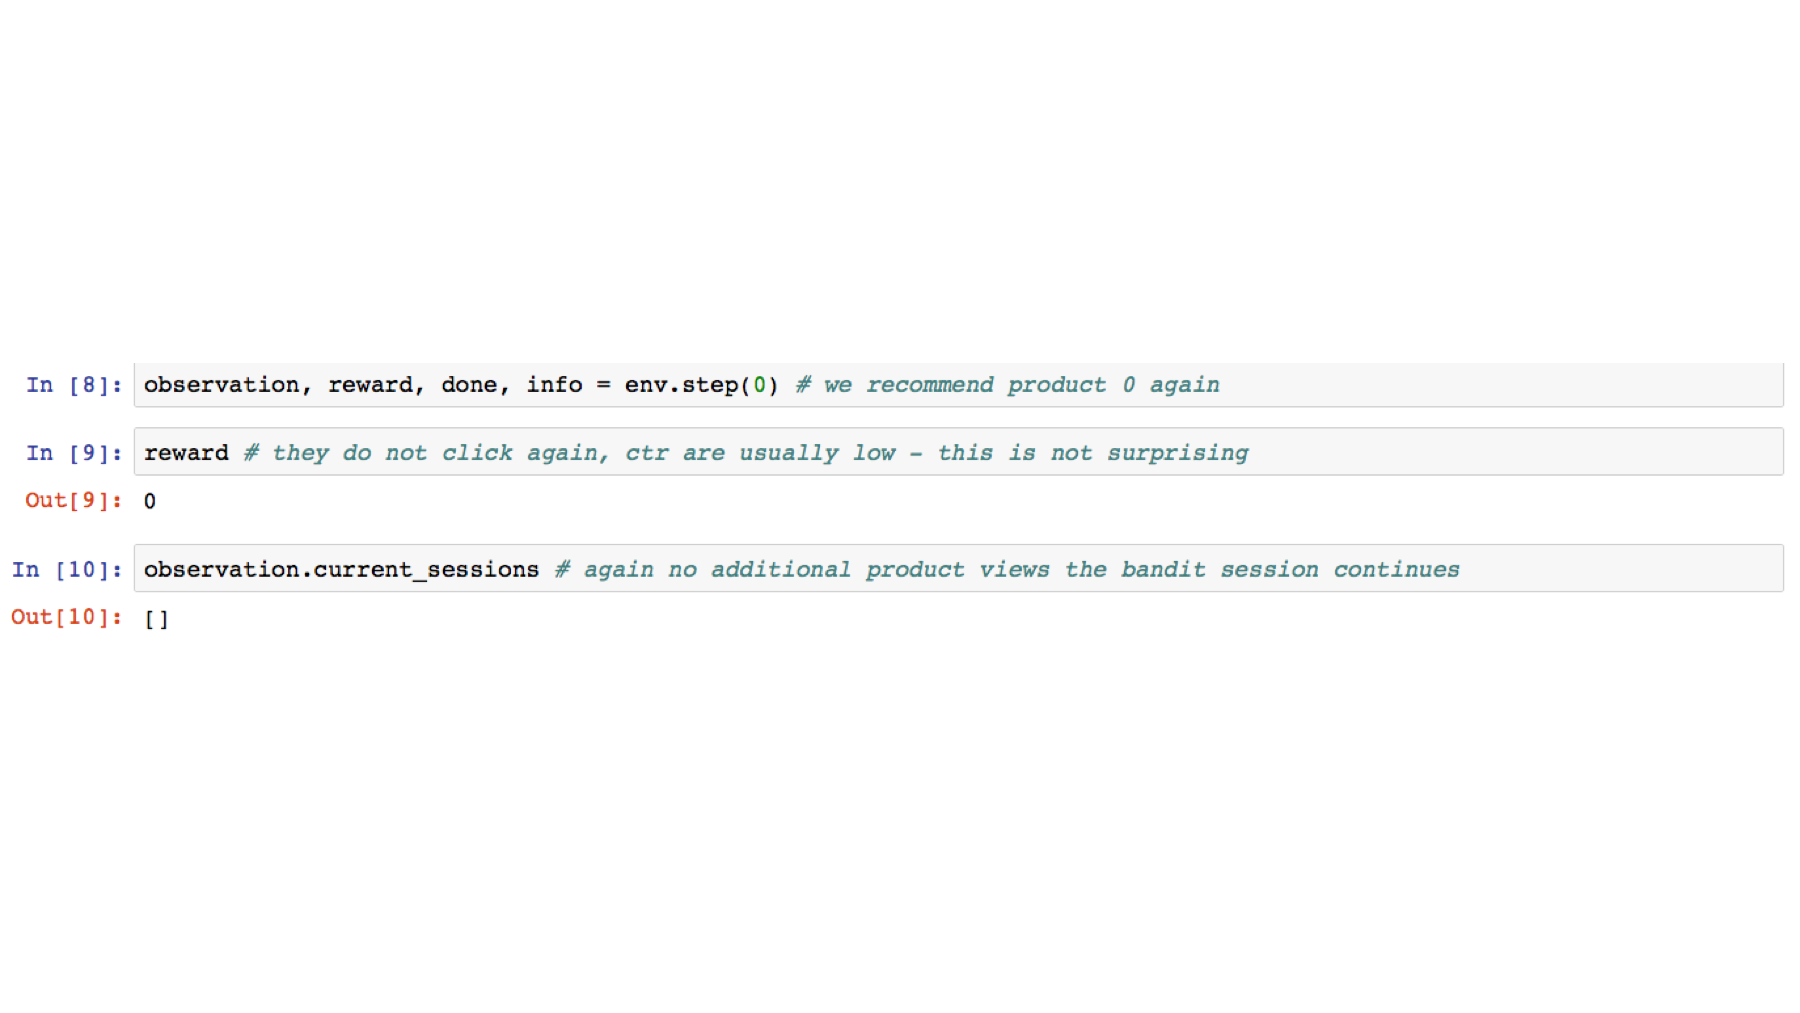
\includegraphics[scale=0.3]{images/reco_gym_sess2.png}
       \centering
       \label{motex1}
   \end{figure}
     
 \end{frame}



 \begin{frame}
  \frametitle{The RecoGym Session}
 
 
   \begin{figure}[h!]
     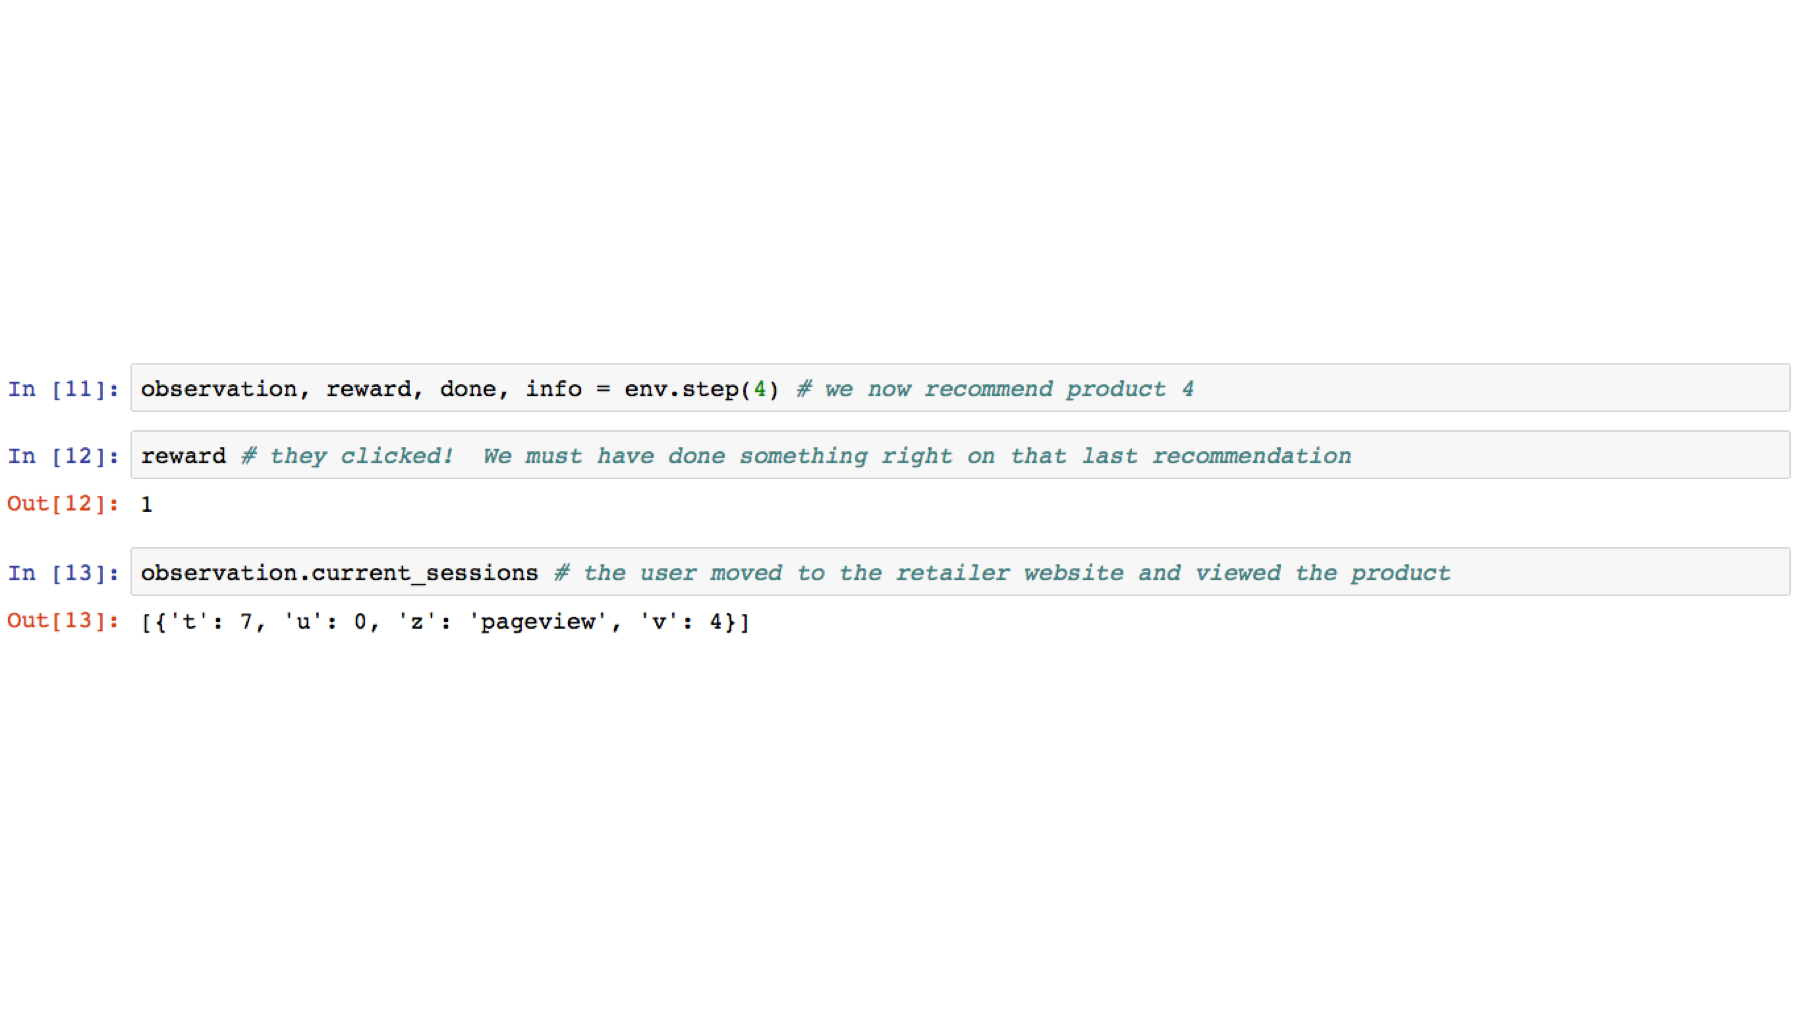
\includegraphics[scale=0.3]{images/reco_gym_sess3.png}
       \centering
       \label{motex1}
   \end{figure}
\end{frame}



   \begin{frame}
    \frametitle{Unlike RL we continue to use logs}
   
    Let's start with a random logging policy (a crazy thing to do, but a useful theoretical concept).
    
     \begin{figure}[h!]
       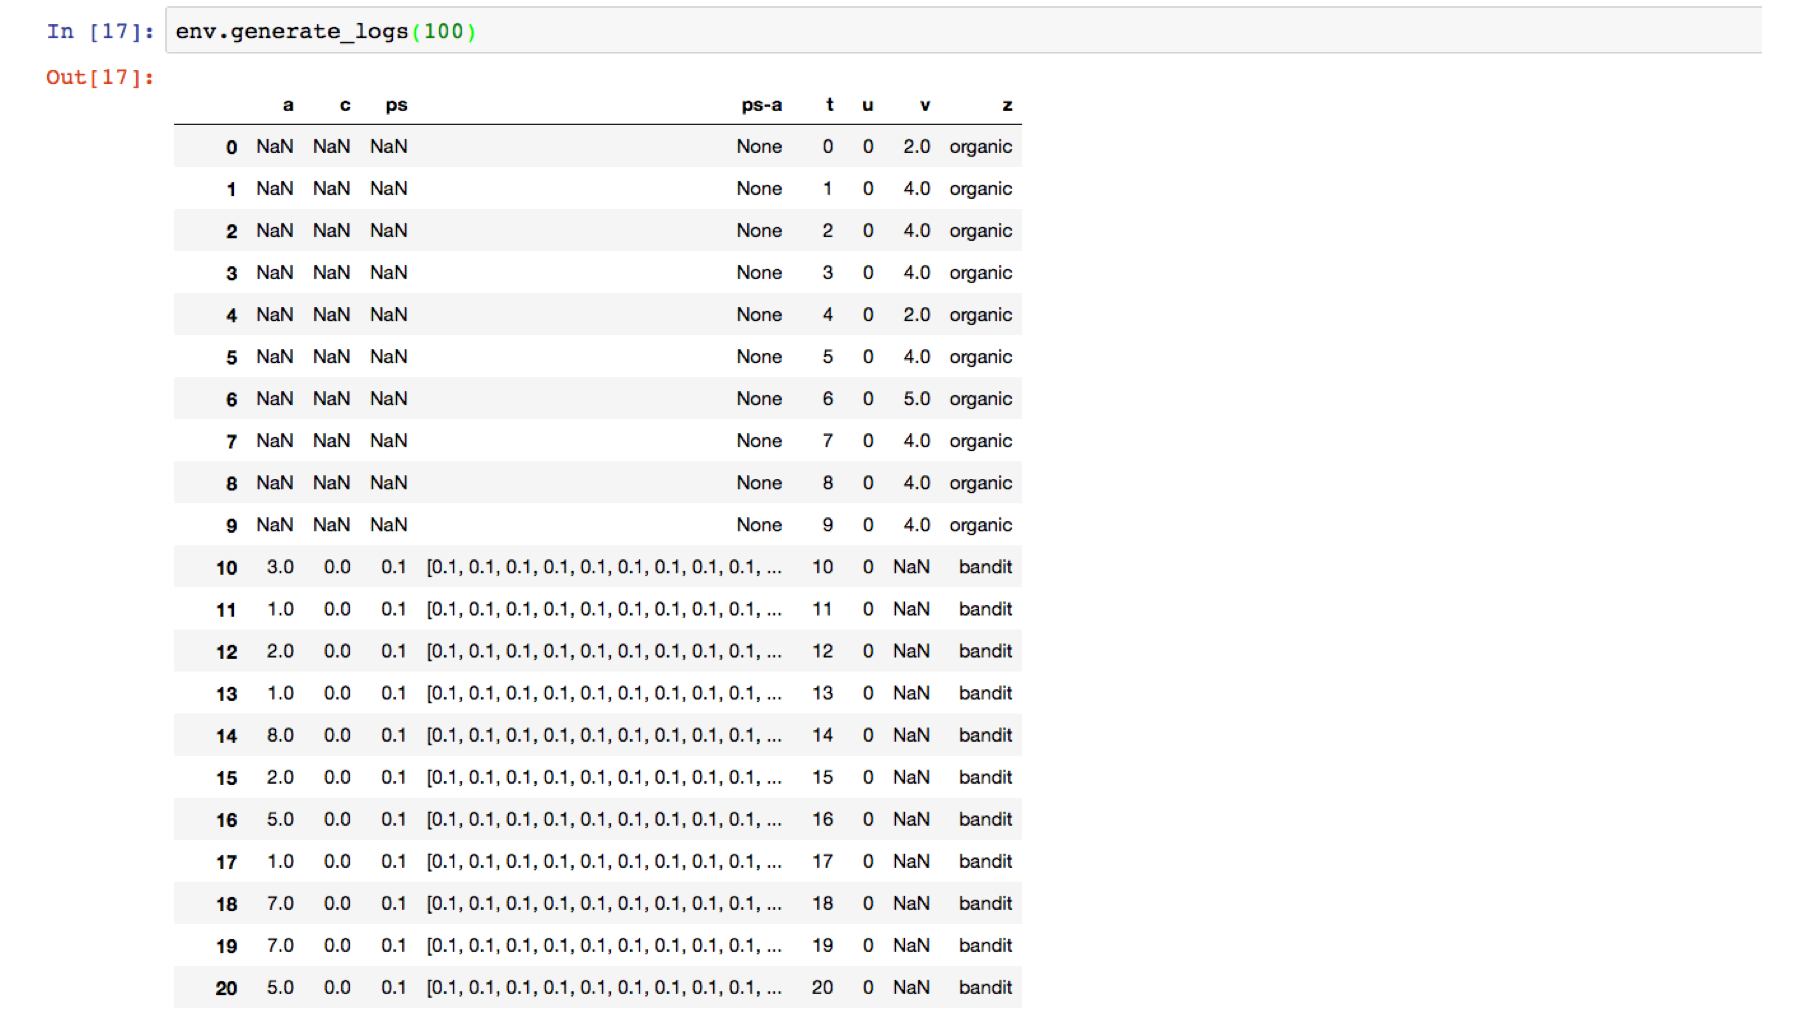
\includegraphics[scale=0.3]{images/recogymlog.png}
         \centering
         \label{motex1}
     \end{figure}
  \end{frame}

\plain{Organic Best Of vs Bandit Best Of}

  \begin{frame}
    \frametitle{Exercise - Getting Started with RecoGym}

    Go to the notebook ``Module III A.ipynb'' \href{https://colab.research.google.com/github/criteo-research/reco-gym/blob/DS3/Module\%20III\%20A.ipynb}{Click Here}

\begin{itemize}
  \item Examine the logs, to start with we will look at non-personalized behavior only.
  \item Plot a histogram of organic product popularity. What is the most popular product?  
  \item Plot the (non-personalized) click through rate of each product (with an error analysis).  What is the most clicked-on product?
  \item Plot popularity against click through rate.  How good a proxy is popularity for click through rate?
  \item Simulate an AB test comparing a simple recommender system (agent) that always recommends the highest ctr product with a recommender system that always recommends the organically most popular product.
\end{itemize}

\end{frame}

\begin{frame}
  \frametitle{Harder questions}

Reflect on how the logging policy would affect these results.

\pause

What is personalization? What impact does personalization bring?

\pause

Where does traditional academic recommender systems research fit into this picture?  

\end{frame}

\plain{Evaluate an organic agent using the Bandit Signal}

\begin{frame}
  \frametitle{The cold start scenario}

    \begin{itemize}
      \item You need to build a recommender system for a client, they have an existing system with existing organic traffic.  \pause This means you can build standard next item predictions to build models of user behavior and understand how user's preferences cluster together. \pause
      \item They are currently running a recommender system with a random policy. \pause
      \item Your task is to build a next item prediction model as a proxy for a recommendation algorithm.  Then produce offline metrics to convince the engineering team to run an AB test.\pause
      \item Finally you evaluate your performance against production.
    \end{itemize}

    \pause
    Please look at notebook ``Module III B.ipynb''   \href{https://colab.research.google.com/github/criteo-research/reco-gym/blob/DS3/Module\%20III\%20B.ipynb}{Click here}


\end{frame}



\plain{Likelihood Based Agents}

\begin{frame}
  \frametitle{Likelihood Based Agent}

  \[
    c_n \sim {\rm Bernoulli}
      \left(
        \sigma
          \left(
      \bPhi {\left( [\bX_n ~ \ba_n] \right)}^T \bbeta
          \right)
      \right)
    \]

    where
    \begin{itemize}
      \item $\bbeta$ are the parameters;
      \item $\sigma \left( \cdot \right)$ is the logistic sigmoid;
      \item $\bPhi \left( \cdot \right)$ is a function that maps $\bX,\ba$ to a higher dimensional space and includes some interaction terms between ${\bX}_n$ and ${\ba}_n$. \pause \emph{Why?}
    \end{itemize}
    


\end{frame}

\begin{frame}
  \frametitle{Likelihood Based Agent}

Or using $\bPhi \left( \left[ {\bX}_n ~ {\ba}_n \right] \right) = {\bX}_n \otimes {\ba}_n$:

\begin{align*}
	\hat{\bbeta}_{\rm lh} = {\rm argmax}_{\bbeta}
	& \sum_n c_n \log \sigma
				\left(
					{
						\left(
							{\bX}_n \otimes {\ba}_n
						\right)
					}^T \bbeta
				\right) \\
	& + \left(
		1-c_n
	  \right)
	  \log
	  \left(
	  	1 - \sigma
			\left(
				{
					\left(
						{\bX}_n \otimes {\ba}_n
					\right)
				}^T \bbeta
			\right)
	\right)
  \end{align*}
\end{frame}


\begin{frame}
  \frametitle{Feature Engineering to get the context vector $\bX$}

  The above model requires us to specify the context $\bX$, how can we do this?
\end{frame}




\begin{frame}
  \frametitle{Feature Engineering}
 
 
   \begin{figure}[h!]
     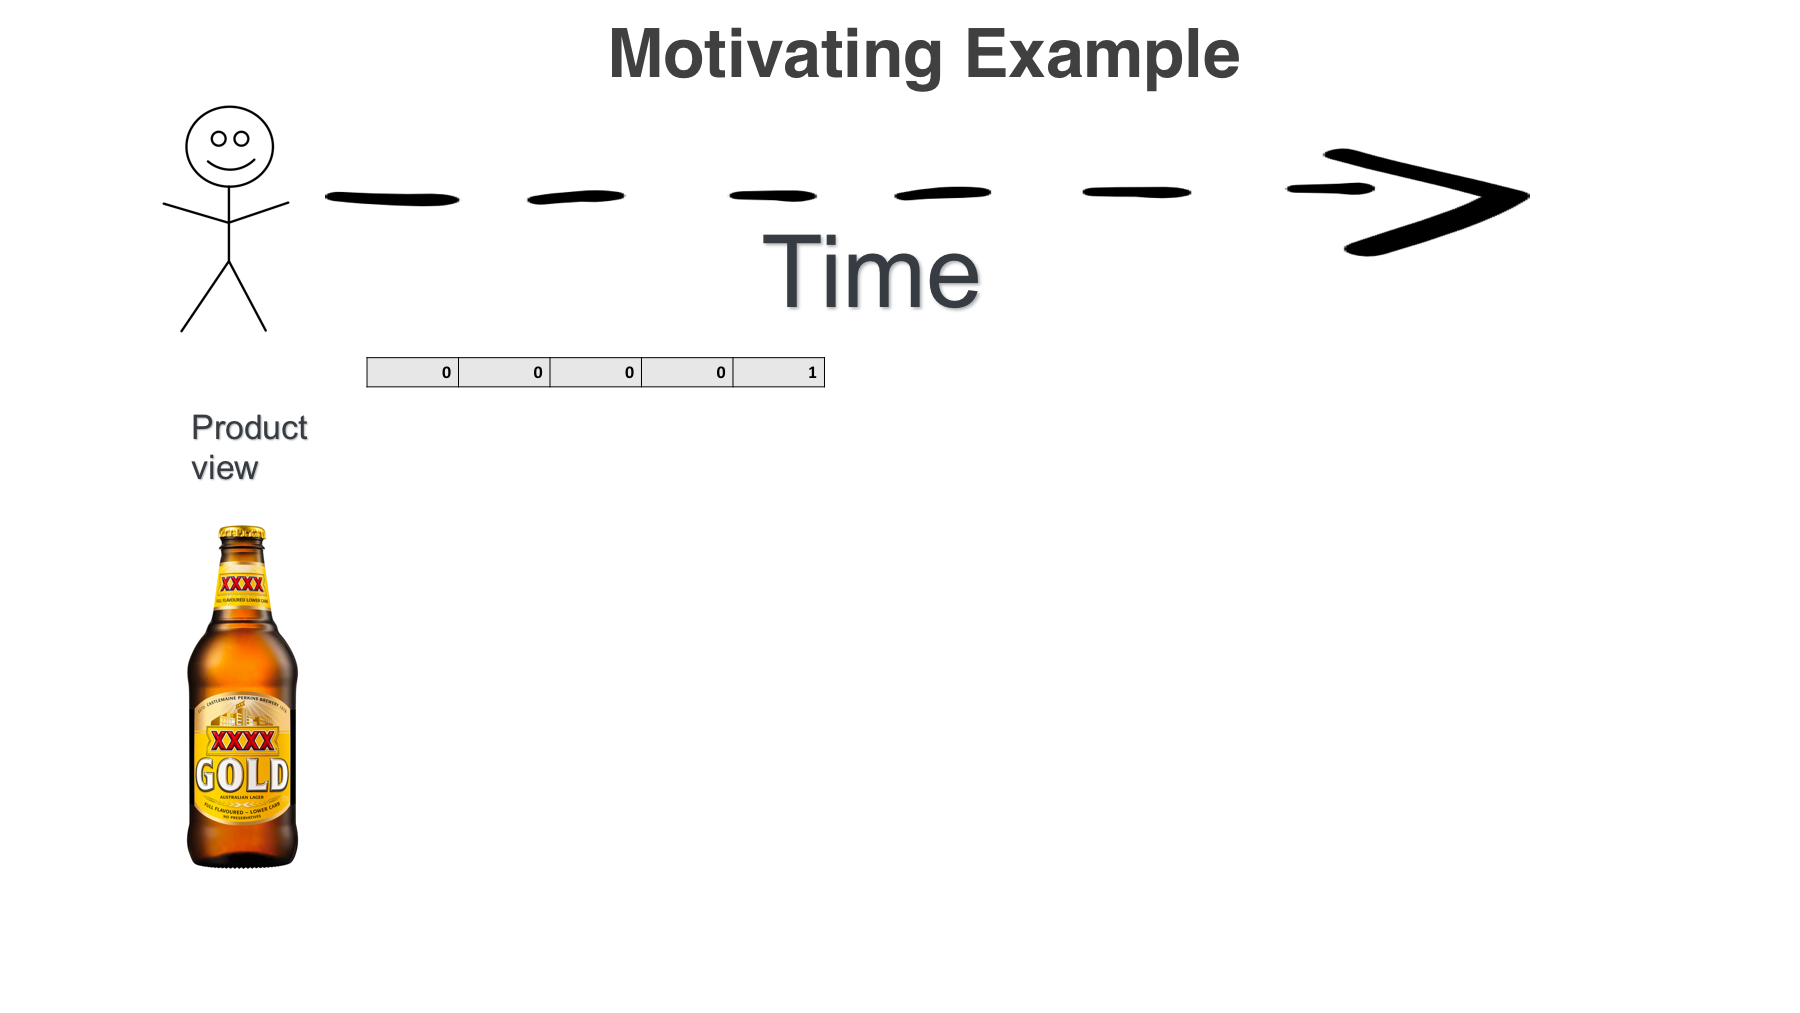
\includegraphics[scale=0.25]{images/feat_eng1.png}
       \centering
       \label{motex1}
   \end{figure}
     
 \end{frame}


 \begin{frame}
  \frametitle{Feature Engineering}
 
 
   \begin{figure}[h!]
     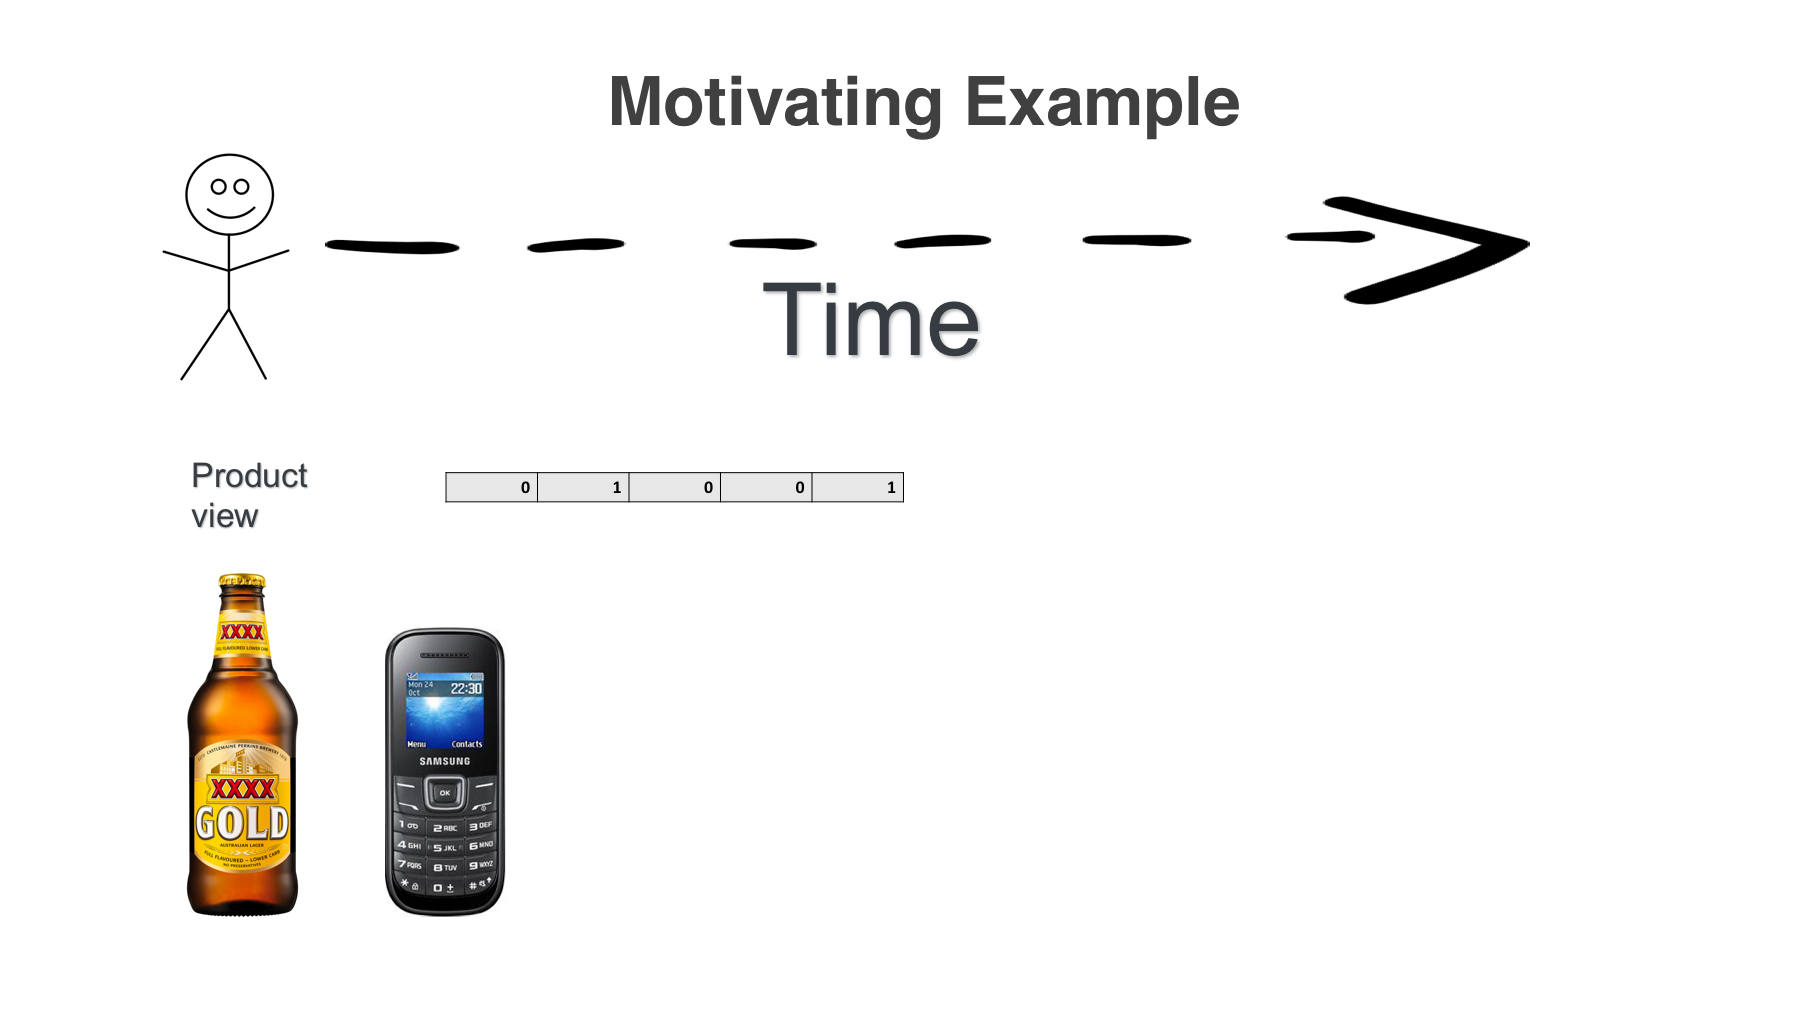
\includegraphics[scale=0.25]{images/feat_eng2.png}
       \centering
       \label{motex1}
   \end{figure}
     
 \end{frame}

 \begin{frame}
  \frametitle{Feature Engineering}
 
 
   \begin{figure}[h!]
     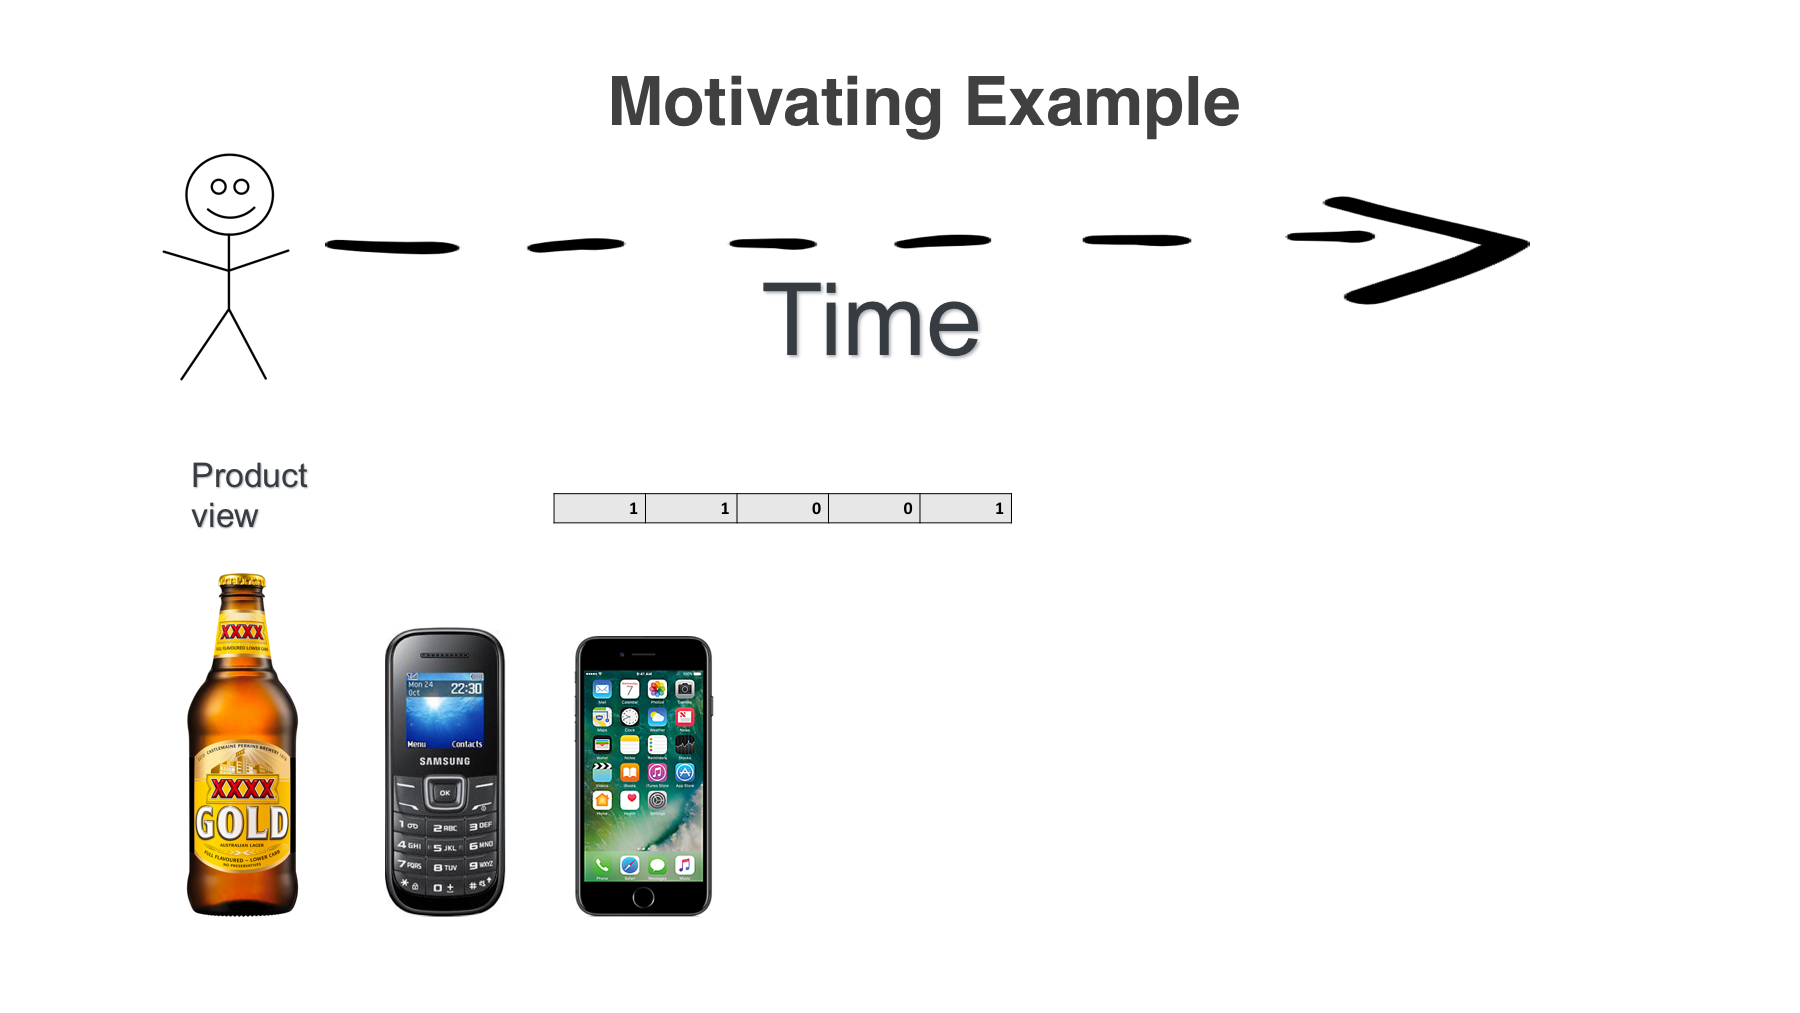
\includegraphics[scale=0.25]{images/feat_eng3.png}
       \centering
       \label{motex1}
   \end{figure}
     
 \end{frame}

 \begin{frame}
  \frametitle{Feature Engineering}
 
 
   \begin{figure}[h!]
     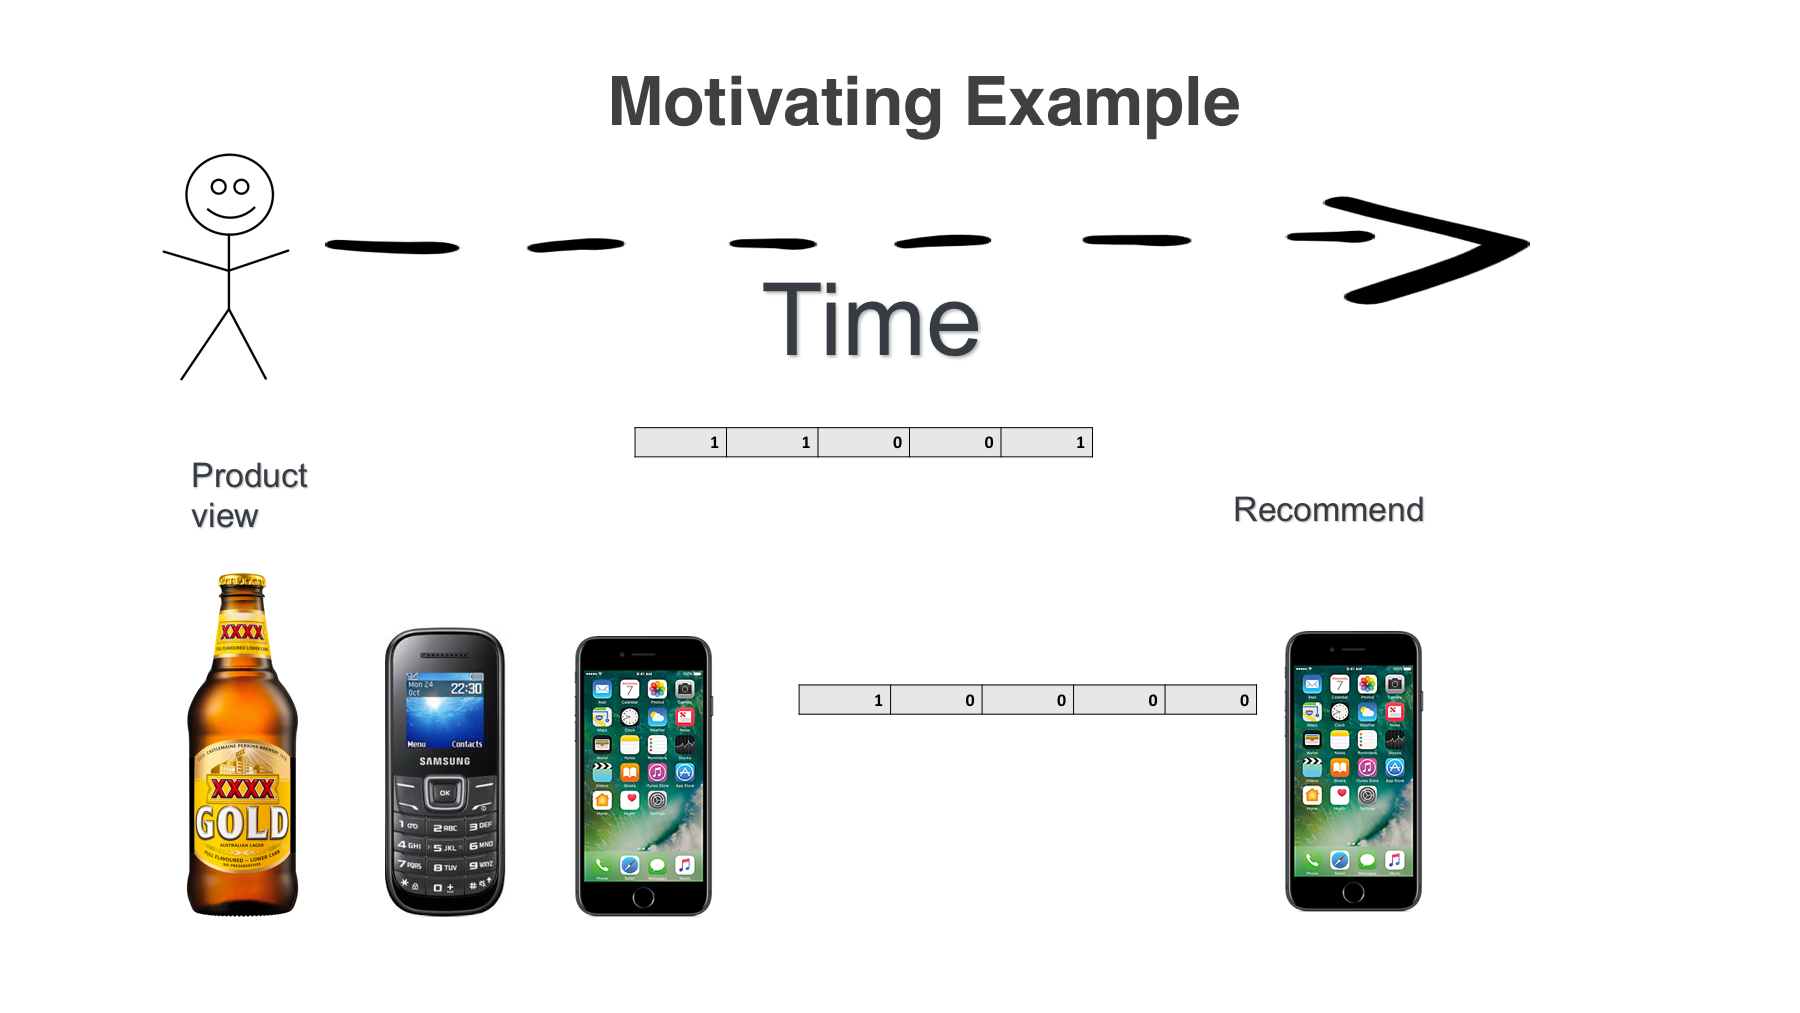
\includegraphics[scale=0.25]{images/feat_eng4.png}
       \centering
       \label{motex1}
   \end{figure}
     
 \end{frame}



\begin{frame}
  \frametitle{Feature Engineering}
\begin{figure}[h!]
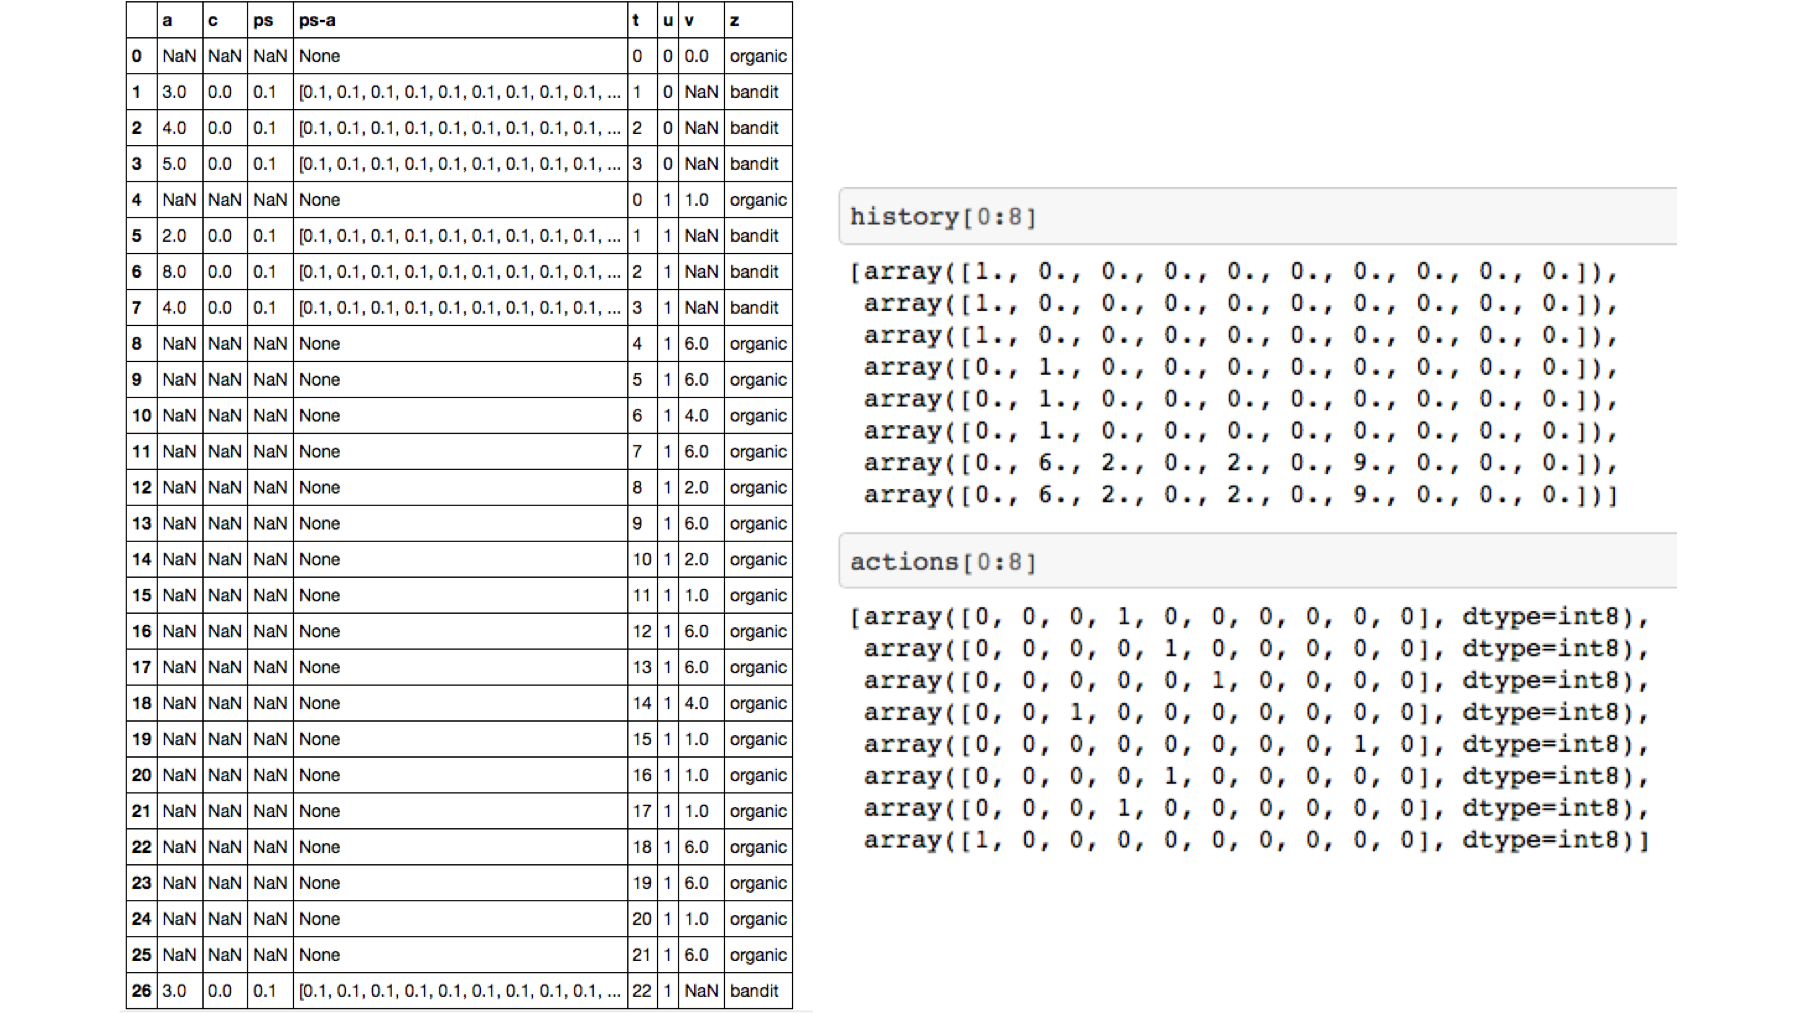
\includegraphics[scale=0.3]{images/feature_engineering.png}
\centering
\end{figure}

\pause
How would you interact the features?

\pause
Is this a good feature engineering scheme?  Can you improve it?
\end{frame}




\begin{frame}
  \frametitle{Pure Bandit Feedback}

    \begin{itemize}
      \item Build a model using feature engineering using logistic regression (or a deep model) \pause
      \item Finally you evaluate your performance against production.
    \end{itemize}

    \pause
    Please look at notebook ``Module III C.ipynb''
    \href{https://colab.research.google.com/github/criteo-research/reco-gym/blob/DS3/Module\%20III\%20C.ipynb}{Click here}


    \pause
    What is lacking in this approach?

\end{frame}




\plain{Combining Organic Signal with Bandit Signal}


\begin{frame}
  \frametitle{Pure Organic vs Pure Bandit}
\begin{figure}[h!]
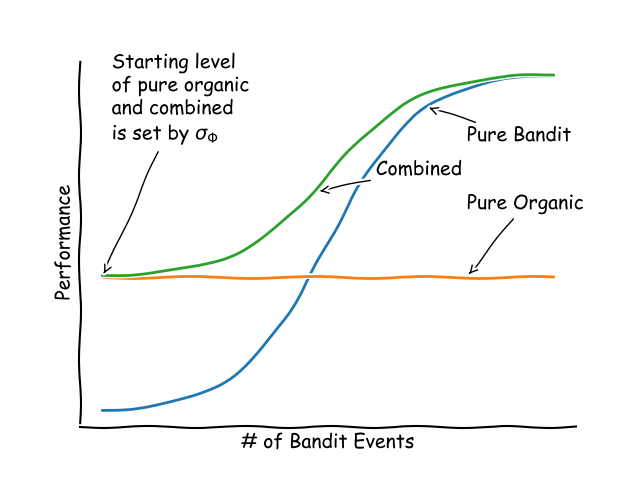
\includegraphics[scale=0.45]{images/pureorganicpurebandit.png}
\centering
\end{figure}
\end{frame}






\begin{frame}
  \frametitle{Can we get the best of both worlds?}

A simple algorithm:

\pause
Use one of the methods from the first part of the course on the organic data to prouduce product embeddings.  Classic methods are SVD or word2vec.

\pause

A user's history is then a list of embeddings rather than non-descript identifiers.

\pause

The action space is also in the same embedding space.

\pause

Exercise: implement this approach, use module III B and C as a reference.

\pause

\emph{What advantages or challenges do you have in this approach?}
\end{frame}
